%%%%%%%%%%%%%%%%%%%%%%%%%%%%%%%%%%%%%%%%%%%%%%%%%%%%%%%%%%%%%%%%%%%%%%%%%%%%%%%%
%2345678901234567890123456789012345678901234567890123456789012345678901234567890
%        1         2         3         4         5         6         7         8

\documentclass[defaultstyle,12pt]{proposal}
%\usepackage{times}

% Usual setup packages
\usepackage{listings} % For including source code with highlighting
\usepackage[bottom]{footmisc} % places footnotes at page bottom

% Packages for verbatim text blocks
\usepackage{alltt} % Package for including math in verbatim text
\usepackage{fancyvrb}

% Packages for math symbols and other mathey things
\usepackage{amsthm}
\newtheorem{theorem}{Theorem}
\newtheorem{lemma}{Lemma}
\newtheorem{claim}{Claim}
\newtheorem{corollary}{Corollary}
\newtheorem{proposition}{Proposition}
\usepackage{amsmath}
\usepackage{amsfonts}
\usepackage{amssymb}
\usepackage{enumerate}
\usepackage{mathtools}

% Packages for including pseudo-code
\usepackage{algorithmicx}
\usepackage{algorithm}
\usepackage{algpseudocode}

% Packages that handle tables, figures and other floats
\usepackage{tabularx}
\usepackage{multirow}
\usepackage{float} % To make floats movable
\usepackage{subcaption}
\usepackage[table]{xcolor}

% For cleaner citations
\usepackage{cite}

% Packages for drawing graphs, FSMs, etc.
\usepackage{pgf}
\usepackage{tikz}
\usetikzlibrary{shapes,arrows,calc,fit,positioning,shapes.symbols,shapes.callouts,patterns,automata,matrix}

% To keep footnotes on the same page are reference
\interfootnotelinepenalty=10000
\raggedbottom

% ------------------------------ CUSTOM MACROS ------------------------------------
% Nice little macro for adding a comment box. Include incrementing comment numbers.
\newcounter{comcount}
\setcounter{comcount}{0}
\newcommand{\mycomment}[1]
{
\refstepcounter{comcount}
\smallskip\noindent\fbox{\parbox{\linewidth}{\emph{Comment \arabic{comcount}} : \small{#1}}} 
}

% - Math
\DeclareMathOperator*{\argmin}{\arg\!\min\>}
\newcommand{\amin}[1]{\underset{#1}\argmin}
\DeclareMathOperator*{\argmax}{\arg\!\max\>}
\newcommand{\amax}[1]{\underset{#1}\argmax}
\DeclarePairedDelimiter\ceil{\lceil}{\rceil}
\DeclarePairedDelimiter\floor{\lfloor}{\rfloor}

\newcommand{\V}[1]{\mathbf{#1}}
\newcommand{\D}[2]{\frac{d#1}{d#2}}
\newcommand{\abs}[1]{\lvert#1\rvert}
\newcommand{\norm}[1]{\lVert#1\rVert}
\newcommand{\ubar}[1]{\underline{#1}}
\newcommand{\vnorm}[1]{\left|\left|#1\right|\right|}
\newcommand{\PD}[2]{\frac{\partial #1}{\partial #2}}

\def\a{\mathbf{a}}    % Action profile
\def\Z{\mathbb{Z}}    % Integers
\def\R{\mathbb{R}}    % Reals
\def\N{\mathcal{N}}   % Naturals
\def\td{\mathbf{t}}   % Response-threshold value
\def\xm{x_{\hat{m}}}  % Agent team size estimate
\def\Ac{\mathcal{A}}  % (Bayesian) Action Profile
\def\St{\mathcal{S}}  % (Bayesian/Extensive) State List, Strategy set
\def\Pl{\mathcal{N}}  % (Extensive/Bayesian) Player List
\def\Hi{\mathcal{H}}  % (Extensive) Game History
\def\Pf{\mathcal{P}}  % (Extensive) Player Function
\def\Th{\mathcal{Z}}  % (Extensive) Terminal History
\def\Ta{\mathcal{T}}  % (Cooperative) Targets/Resources
\def\Co{\mathcal{C}}  % (Cooperative) Player assignment constraints
\def\sig{\mathcal{S}} % Sigmoid function

% ------------------------------ DOCUMENT TITLE SETUP -------------------------
\title{Optimal Task-Assignment in Multi-Agent Systems}

\author{A.~P.}{Kanakia}

\otherdegrees{B.S., University of Illinois at Urbana-Champaign, 2010\\
	      M.S., University of Colorado, Boulder, 2014}

\degree{Doctor of Philosophy}		%  #1 {long descr.}
	{Ph.D., Computer Science}		%  #2 {short descr.}

\dept{Department of}			%  #1 {designation}
	{Computer Science}		%  #2 {name}

\advisor{Prof.}				%  #1 {title}
	{Nikolaus Correll}			%  #2 {name}

\reader{Prof.~Ani Hsieh}		%  2nd person to sign thesis
\readerThree{Prof.~Behrouz Touri}		%  3rd person to sign thesis
\readerFour{Prof.~Gabe Sibley}
\readerFive{Prof.~Sriram Sankaranarayanan}

\abstract{  %\OnePageChapter	% because it is very short
	For my dissertation proposal I present a novel methodology for task-assignment in multi-agent systems. I propose using response-threshold models (both discrete and continuous) for making agent-level decisions to control macroscopic system-level behavior---drawing inspiration from social insect models such as ant colonies and bee hives. The use of such models is not new in the field of swarm robotics. Phenomenological evidence from ethologist research has provided ample evidence of the success of threshold based models for task-assignment in a multi-agent system and many swarm robotics researchers have adopted and adapted these models to engineer cooperative robotic systems.
	
	My contribution provides a natural extension to response-threshold models to account for dynamic tasks which require varying group sizes. I achieve this through the use of agent-level sigmoid functions, particularly the logistic function which can be tuned using a pair of parameters mapping to the desired system-level mean and variance of team sizes. I then show that response-threshold functions are a particularly good tool for solving the problem of collaborative task-assignment by proving equilibrium properties of the system resulting from their use. 
	
	Finally, I propose a modeling framework for optimal control of a swarm system using response-threshold based task-assignment. I explain what the term \emph{optimal control} means in the context of multi-agent task-assignment. My current goal is to set up a specific closed-loop control experiment for parameter identification and optimization using simulations and models at different layers of abstraction (micro, macro and physical layers). I also discuss avenues for future research including distributed multi-agent optimization and game theory reformulations of the problem being studied. My research does not focus on the physical limitations/constraints of robotic hardware to perform the required dynamic tasks, although I have played a large part in the design and construction of the Droplet swarm robot platform that I will use for my experiments. The target application for my dissertation work will be distributed indirect parameter based control of a swarm of capable robots to complete dynamic cooperative tasks with minimal human intervention.
	}

\dedication[Dedication]{	% NEVER use \OnePageChapter here.
	TBD
	}

\acknowledgements{	\OnePageChapter	% *MUST* BE ONLY ONE PAGE!
	TBD
	}

%\ToCisShort	% use this only for 1-page Table of Contents

%\LoFisShort	% use this only for 1-page Table of Figures
% \emptyLoF	% use this if there is no List of Figures

%\LoTisShort	% use this only for 1-page Table of Tables
 \emptyLoT	% use this if there is no List of Tables

% ----------------------------- BEGIN DOCUMENT --------------------------------
\begin{document}
%%%%%%%%%%%%%%%%%%%%%%%%%%%%%%%%%%%%%%%%%%%%%%%%%%%%%%%%%%%%%%%%%%%%%%%%%%%%%%%%
\chapter*{Acronyms}
\begin{itemize}
	\item \textbf{CRT}: Continuous Response-Threshold
	\item \textbf{DRT}: Discrete Response-Threshold
	\item \textbf{MAS}: Multi-Agent System
	\item \textbf{ODE}: Ordinary Differential Equation
	\item \textbf{PFSM}: Probabilistic Finite State Machine
	\item \textbf{RT}: Response-Threshold
	\item \textbf{TA}: Task-Assignment or Task-Allocation (used synonymously)
\end{itemize}

%%%%%%%%%%%%%%%%%%%%%%%%%%%%%%%%%%%%%%%%%%%%%%%%%%%%%%%%%%%%%%%%%%%%%%%%%%%%%%%%
\chapter{Introduction}
Many social, biological and physical systems can be represented as swarm systems. From modeling human societal interaction and population dynamics to insect colonies and great animal herd migrations, from cellular automata to distributed network systems and even the interconnected computing devices that form the internet can be viewed as swarm intelligence. Swarm robotics \cite{Sahin2005} is a branch of swarm intelligence applied to physical multi-agent systems (MAS) to leverage the advantage of producing emergent, complex behavior from individually simplistic agents and rules. This has led to novel approaches in the design and analysis of MAS and the algorithms associated with them \cite{Brambilla2013}.

Swarm systems have many benefits over traditional, centralized robot systems. The robots used in swarm applications are generally many orders of magnitude smaller (cm vs.~m, grams vs.~kg) and simpler in design ($<10$ vs.~$100$s of actuators) than conventional robots, while being much greater in number ($10^2$ to $10^{<<23}$). Also, most swarm systems are homogeneous---robots with identical software/hardware are used to complete the assigned task. This makes swarm systems easily scalable while simultaneously keeping manufacturing and maintenance costs of the hardware low. Though, perhaps their greatest advantage is system stability and robustness to error. Most swarm systems consist of small, relatively simple robots that are only capable of limited and noisy sensing, communication and actuation. This means that while no single robot alone is capable of performing the task assigned, the system as a whole is resilient to individual unit errors and is capable of completing the task \cite{Winfield2005}.

Swarm robotics has tackled a vast array of MAS problems in the past two decades. It's corpus ranges from self-organization, self-assembly, pattern formation, and aggregation to foraging, coordinated movement (such as flocking and schooling), and group surveillance. Readers are directed to \cite{Bayindir2007} and the references therein for further information on any of these topics. 

Performing collaborative tasks is a vast sub-field of study in swarm robotics and considerable work has been done to understand and model such scenarios, particularly by \cite{Martinoli1995, Martinoli1999b, Agassounon2001, Ijspeert2001, Agassounon2002} using the well known stick-pulling experiments. Collaborative tasks using MAS extend to a variety of potential real-world applications such as oil-spill containment, firefighting (particularly large forest fires), object transport, and group surveillance. Am important question that has so far remained unanswered when attempting collaborative tasks is how many agents are required to complete a given task of a certain size and how are they recruited? It is often assumed that all robots are pre-programmed to form groups of a particular size beforehand or that the task requires an \emph{exact} number of robots to complete successfully---a number that is known beforehand.

\begin{figure}[!tb]
	\centering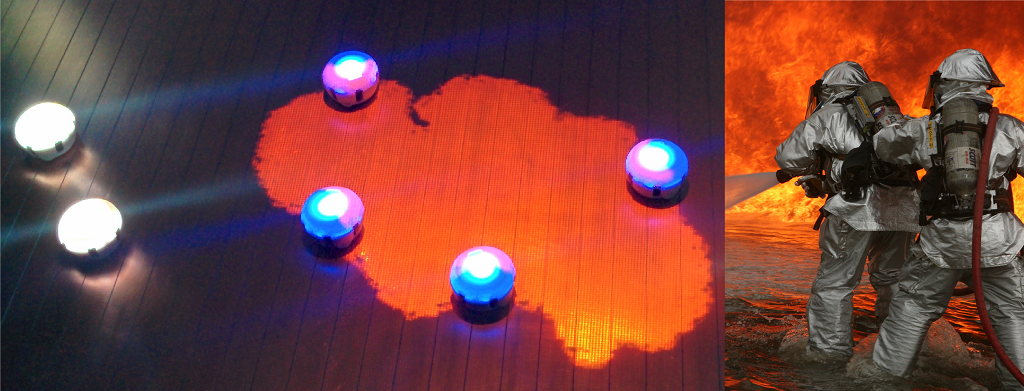
\includegraphics[width=\textwidth]{../assets/dropletfire.png}
	\centering\caption{The \emph{Droplet} swarm robots running a fire containment experiment inspired by a real forest firefighting scenario.}\label{fig:dropletfire}
\end{figure}

But what about tasks that are dynamic in nature such as fighting forest fires? In such cases it is impractical and often impossible to know beforehand, exactly how many agents are required for successful completion. More importantly, the benefit of larger teams of agents for such collaborative tasks increases non-linearly with team size, e.g. Where 1-5 robots may be incapable of lifting a heavy object, 6-7 will be able to lift and move it successfully but the usefulness more than 7 robots begins to diminish rapidly thereafter. I define such tasks with non-linear increase in system utility with increasing team sizes as \emph{concurrent benefit} tasks. It is for such situations that I propose a novel methodology for estimating group sizes in a distributed fashion, as described below.

\emph{Empirical evidence from biological systems suggests that there exists a generalized solution for collaborative task-assignment in multi-agent systems. This solution involves the use of response-threshold functions which leads to a system-level equilibrium and can be used for optimal control of a multi-agent system.}

The rest of the paper is organized as follows. Section~\ref{sec:relwork} describes related work in multi-agent TA from multiple disciplines including Biology, Swarm Robotics, and Game Theory. The discussion in this section outlines the evolution of the TA problem from being a model  for describing social systems such insect colonies to an engineering approach for programming artificial multi-agent systems such as robot swarms. Chapter~\ref{ch:background} provides an outline of existing swarm modeling techniques, particularly multi-level abstraction using probabilistic finite state machines (PFSMs) and rate equations. Readers familiar with these techniques may skip this tutorial chapter and move straight to Chapter~\ref{ch:resthmodel}. Here, I introduce the continuous response-threshold (CRT) model for TA that is central to my study. The CRT model involves agents using a logistic function with two tunable parameters to control the mean and variance of desired team size formation. I analyze and verify this model using real robot experiments as well as simulation results. The widespread success and relevance of RT models in many disciplines led me to investigate their properties which, in turn, led to the development of two theorems showing existence of system-level equilibria for these models. This investigation forms the basis of Chapter~\ref{ch:existeqrtm}. Due to a heavy reliance on game theory formalism for proofs of the two theorems, Section~\ref{sec:ggoverview} of provides a brief introduction to the theory of \emph{global games}. The final chapter of my proposal discusses future/proposed work for my dissertation in the form of a generalized model for MAS control. Using the results from the previous two chapters I propose a novel parameter discovery and optimization methodology for swarm robot control. Finally, the Conclusion chapter briefly reiterates the original contribution my dissertation will provide for the field of swarm robotics.


\section{Related Work}\label{sec:relwork}
Using RT functions to model social behavior in insects such as ant colonies \cite{Bonabeau1996, Bonabeau1997} and bee hives \cite{Robinson1987, Robinson1992, PageJr1990} has been proposed, analyzed and verified by biologists since the 1980's \cite{Theraulaz1998}. In the past two decades swarm roboticists have begun to engineer MASs using these models. Jones and Matari\'c \cite{Jones2004} describe an adaptive method of TA for a large-scale minimalist robot system where agents independently switch between picking up different colored pucks to maintain a consistent rate of foraging for each type of colored puck. While the authors do not directly reference threshold functions, their switching algorithm simply assigns probabilities of picking up a certain colored puck versus another by accounting for the number of colored pucks observed by a robot around it, which is a form of probabilistic threshold policy. Such dynamic probabilistic threshold policies are also studied in \cite{Nouyan2002}. I proposed a modification of such strategies to instead use the logistic sigmoid function \cite{Kanakia2014}. Using a logistic function better exposes mean and variance parameters of the resulting team sizes for CRT functions. These two parameters, along with the number of workers available and the manner in which they acquire information, are the building blocks governing TA behavior of an agent in the collective swarm (see section titled, ``Division of Labor as a Self-Organizing Process'' in \cite{Robinson1992}).

All of the aforementioned work uses CRT functions. In contrast to this, DRTs (such as step-functions) for TA and recruitment have been studied by a number of research groups utilizing the \emph{stick pulling} experiment \cite{Martinoli1995, Martinoli1998, Lerman2001, Martinoli2004}. Here, a task can only be solved with an exact number of robots $= \td$. The problem of distributing a swarm of robots across multiple sites with a specific desired distribution has been studied in \cite{Berman2009, Correll2008} and is extended by Mather \cite{Mather2010} allowing assignment to tasks requiring a varying number of robots. The benefits of using a TA algorithm versus just allowing agents to attempt a collaborative task, such as aggregation, without a RT is analyzed in \cite{Agassounon2001}. The authors show that threshold based TA results in increasing aggregation of seeds while no TA results in stagnation of seed collection after a little while. 

I have shown in \cite{Kanakia2014} (see Chapter~\ref{ch:resthmodel}) that the DRT strategy is a special case of CRTs when the slope of the sigmoid threshold function approaches infinity, and thus the step-function behavior can be accurately reproduced by the latter. In practice, varying the slope of the RT function allows us to balance exploration and exploitation in the system \cite{Bonabeau1997}. It is worth noting that biological systems do not necessarily implement sigmoid functions but that they might naturally emerge from a combination of a DRT and noise in the perception system, which I show analytically in \cite{Kanakia2015} (See Chapter~\ref{ch:existeqrtm}). 

The development of multi-agent TA draws a very clear picture of its evolution from a behavioral model for insect colonies, developed by ethologists, to an inspired algorithmic model for adaptive MASs \cite{Krieger2000}. While biologists have provided ample empirical evidence to the success of the RT model in predicting and matching observed swarm behavior for TA, there has been no formal argument as to why natural systems gravitate towards this approach compared to other TA strategies such as leader-follower algorithms \cite{Chen2011} or market-based approaches \cite{Amstutz2008,Vig2007}; see \cite{Kalra2006} for a comparative study. My aim is to show for the first time that agent-level RT strategies drive a swarm system to some notion of equilibrium and consequently, system-level control which makes them an obvious choice for modeling natural systems and engineering artificial ones.



%%%%%%%%%%%%%%%%%%%%%%%%%%%%%%%%%%%%%%%%%%%%%%%%%%%%%%%%%%%%%%%%%%%%%%%%%%%%%%%%
\chapter{Background on Swarm System Modeling Techniques}\label{ch:background}
This chapter is designed to give the reader an introductory lesson on swarm system modeling approaches widely used by the swarm robotics community. This involves the use of PFSMs to mathematically describe individual agent behavior as well as solving systems of coupled ODEs, often termed \emph{rate equations}, to divine macroscopic level properties of the system. These are common tools of the trade for modeling many different kinds of dynamical systems---not just MAS---and as such, if the reader is familiar with these approaches they are encouraged to skip this chapter and move on to Chapter~\ref{ch:resthmodel}.

The first step in the robot controller design methodology is to describe the swarming task being studied. The general strategy used by each individual agent in the swarm is defined and later translated into a viable microscopic model. A hypothesis for the observed, collective behavior of the swarm is supplied, which is later quantified into a mathematical macroscopic model.

Physical characteristics of the swarm system are generally described in the experiment setup as well. These may include environmental variables such as arena size, agents' properties such as speed, communication and sensing radii, the computation power of each individual in the swarm, etc. This is an important step in identifying important system parameters that affect the outcome of the experiment, versus the environmental and agent based values that can be abstracted away when designing micro and macro-level models.
 
\section{Designing the Controller Construct}
Creating a logic construct---a flowchart, state-machine or algorithm---that describes the desired robot behavior for the given task is an important step in the MAS modeling process. When studying non-spatial models, the robot controller can be characterized by an FSM with a discrete number of states under urgent time-step driven semantics, as seen in Figure~\ref{fig:allfsm}. The states in the FSM ($s_1, s_2, s_3$ \& $s_4$) represent physical states that the robot can be in, such as  \emph{searching}, \emph{waiting}, etc. and can be directly derived from the program code running on the robot. One can think of each state as being an \emph{action} that the robot is currently performing based on stimulus from the environment and other robots. These stimuli can cause a robot to transition from one state to another and are represented as \emph{conditionals} on the edges of the FSM, $c_i$. These conditionals are equivalent to the decision process blocks in the flowchart and can be derived from:
\begin{enumerate}
\item Sensor readings (or stigmergy) and explicit communication, e.g., seeing red light through an rgb sensor or seeing a certain number of robots around you,
\item internal timers, e.g., transition back to search after waiting for 3 seconds,
\item or a combination of both, e.g., transition back to search after waiting for 3 seconds \emph{iff} you see no other robots in your vicinity, otherwise, reset your timer.
\end{enumerate}

I can now extend this modeling framework of robot behavior as an FSM to construct a PFSM, where the conditionals in the FSM are no longer true/false values but instead are probabilities of transitioning from one state to another based on external stimulus or internal state. 

As alluded to earlier, the case of a state transition based on an internal timer is especially interesting. Let $c_1$ in Figure~\ref{fig:fsm} be the condition $t_{s_1} \geq 5$, i.e. time in state $s_1$ is greater than or equal to 5 time steps (or ticks). This conditional is true when the robot has remained in state $s_1$ for at least 5 ticks and consequently transitions to state $s_2$. Thus, the conditional $c_1$ says a robot may remain in state A for no more than 5 ticks. The equivalent transition probability for this condition would be $p_{s_1} = 1/5$. Therefore, at each time step of the PFSM simulation, there is a $1/5$ chance that the robot will transition from state A to state B. The expected number of ticks before a transition happens is then equal to 5. This transition from deterministic FSM models to probabilistic PFSM models for swarm robot algorithms is derived in more detail in \cite{Correll2007}.

\begin{figure}[!tb]
\centering
	\begin{subfigure}[t]{.4\textwidth}
		\centering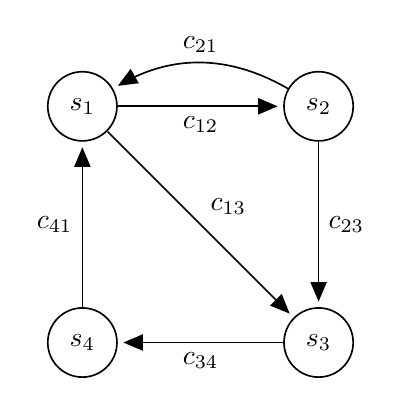
\begin{tikzpicture}[->,>=triangle 45,shorten >=2pt,auto,node distance=3cm,
 	                   semithick]
 	                   
 		 \node[state] (1)              {$s_1$};
 		 \node[state] (2) [right of=1] {$s_2$};
		 \node[state] (3) [below of=2] {$s_3$};
		 \node[state] (4) [below of=1] {$s_4$};

		\begin{scope}
		  \path	 (1) 	edge node[below]{$c_{12}$} (2)
  			          	edge node{$c_{13}$} (3)
				 (2)	edge node{$c_{23}$} (3)
						edge[bend right] node[above]{$c_{21}$} (1)
				 (3) 	edge node{$c_{34}$} (4)	
				 (4) 	edge node{$c_{41}$} (1);
		\end{scope}
		\end{tikzpicture}
	\caption{FSM representing a single robot controller with conditional edge transitions that depend on internal and environmental factors such as timers, sensor readings, etc. Vertices represent physical or internal states that a robot can be in.}\label{fig:fsm}
	\end{subfigure}~
	\begin{subfigure}[t]{.4\textwidth}
		\centering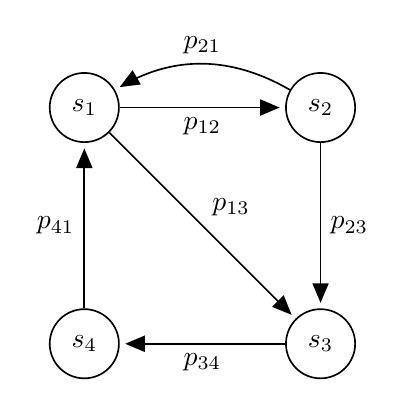
\begin{tikzpicture}[->,>=triangle 45,shorten >=2pt,auto,node distance=3cm,
                    semithick]

 		 \node[state] (1)              {$s_1$};
 		 \node[state] (2) [right of=1] {$s_2$};
		 \node[state] (3) [below of=2] {$s_3$};
		 \node[state] (4) [below of=1] {$s_4$};

		\begin{scope}
		  \path	 (1) 	edge node[below]{$p_{12}$} (2)
  			          	edge node{$p_{13}$} (3)
				 (2)	edge node{$p_{23}$} (3)
						edge[bend right] node[above]{$p_{21}$} (1)
				 (3) 	edge node{$p_{34}$} (4)	
				 (4) 	edge node{$p_{41}$} (1);
		\end{scope}
	\end{tikzpicture}
	\caption{PFSM of a robot controller with probabilistic edge transitions derived from simple geometric properties of the system.}\label{fig:pfsm}
	\end{subfigure}
	\begin{subfigure}[t]{.4\textwidth}
		\centering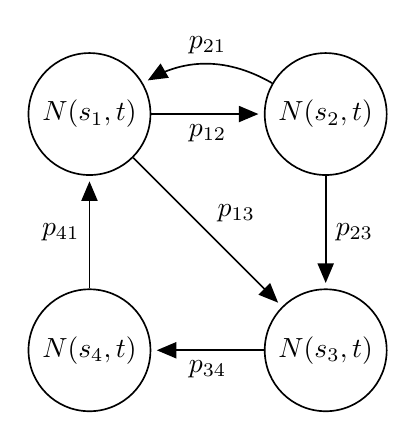
\begin{tikzpicture}[->,>=triangle 45,shorten >=2pt,auto,node distance=3cm,
                    semithick]

 		 \node[state] (1)              {$N(s_1, t)$};
 		 \node[state] (2) [right of=1] {$N(s_2, t)$};
		 \node[state] (3) [below of=2] {$N(s_3, t)$};
		 \node[state] (4) [below of=1] {$N(s_4, t)$};

		\begin{scope}
		  \path	 (1) 	edge node[below]{$p_{12}$} (2)
  			          	edge node{$p_{13}$} (3)
				 (2)	edge node{$p_{23}$} (3)
						edge[bend right] node[above]{$p_{21}$} (1)
				 (3) 	edge node{$p_{34}$} (4)	
				 (4) 	edge node{$p_{41}$} (1);
		\end{scope}
	\end{tikzpicture}
	\caption{A macroscopic model for the swarm system as a whole. Vertices, $N(s_i, t)$, represent the number of robots in state $s_i$ at time $t$. Edges are still transition probabilities between states but can also be thought of as proportions of agents entering or leaving a state at time $t$.}\label{fig:pfsmmacro}
	\end{subfigure}
\caption{Transitioning from, \textbf{(a)}: micro-model FSM that describes a single robot controller, to \textbf{(c)}: macro-model PFSM that characterizes the entire swarm system.}\label{fig:allfsm}
\end{figure}

\section{Mathematical Description of the System}
Given a discrete set of states and conditions for transitions between them, usually in the form of probabilities of transition, a \emph{master equation} defines a set of coupled ODEs that describe the time evolution of a physical system. So far, I have used logical constructs like FSMs to represent the robot controller running within each individual agent of the swarm system. I could instead look as these constructs as a model for the entire system, in which case the vertices of the FSM become accumulators of robots currently in a state and the edges define fractions of agents entering or leaving a given state at time $t$. The PFSM now becomes a macroscopic definition of the robot swarm and can be used to define a mathematical model for the time evolution of the system.

\begin{equation}
\D{\vec{P}(t)} = \mathbf{A}\vec{P}(t)\label{eq:firstmaster}
\end{equation}

$\vec{P}$ is a vector containing the time-dependent probability of being in any given state in the corresponding PFSM. $\mathbf{A}$ is a matrix containing transition rates of going from state-$i$ to state-$j$ in the PFSM. When I multiply both sides of equation~\eqref{eq:firstmaster} by the total number of agents, $N_0$, I get the modified master equation that gives a macroscopic description of the system.
\begin{align}
N_0 \vec{P}'(t) = \mathbf{A}\left(N_0\vec{P}(t)\right)\notag\\
\vec{S}'(t) = \mathbf{A}\vec{S}(t)\label{eq:master}
\end{align}
where $\vec{S}$ is a state vector containing the number of agents in each state, $N_{s_i}$, at time t. Here, $\abs{\vec{S}}$ is equal to the number of unique states of the system, e.g. $\abs{\vec{S}} = 4$ in my previous PFSM example from Figure~\ref{fig:pfsm}. The matrix $\mathbf{A}$ contains transition probabilities between the states in the PFSM. There a two types of elements, $a_{ij}$ in matrix $\mathbf{A}$.
\begin{enumerate}
\item The non-diagonal entries, $a_{ij}$ s.t. $i\not=j$, are equal to $p(c_{ij})$ (shortened to $p_{ij}$), the probability of transitioning from state $s_i$ to $s_j$ via the edge with conditional $c_{ij}$ in the FSM.
\item The diagonal entries, $a_{ii}$, are equal to the negative sum of all edge probabilities $p_{n}$ leaving state $s_i$.
\end{enumerate} 
If an edge does not exist between two states $s_i$, $s_j$ ($i\not=j$) in the FSM, then entry $a_{ij} = 0$, e.g., the master equation for the swarm system described in Figure~\ref{fig:pfsm} is,
\begin{equation}\label{eq:mastereqns}
\left(
	\begin{array}{c}N_A'(t) \\ N_B'(t) \\ N_C'(t) \\ N_D'(t)\end{array}
\right) =
\left(
	\begin{array}{cccc}
	-(p_{12} + p_{13}) & p_{21} & 0 & p_{41}\\
	p_{12} & -(p_{21} + p_{23}) & 0 & 0\\
	p_{13} & p_{23} & -p_{34} & 0\\
	0 & 0 & p_{34} & -p_{41}
	\end{array}
\right)
\left(\begin{array}{c}N_A(t) \\ N_B(t) \\ N_C(t) \\ N_D(t)\end{array}\right)
\end{equation}

In most of the scenarios being discussed in this paper, I assume that agents are neither removed nor added to a swarm system once an experiment has begun and therefore add the following constraints to the model,
\begin{align}
N_0 = & \sum\limits^{\abs{\vec{S}}}_{i=1} N(s_i, t)\\
\forall j \gets 1\ldots\abs{\vec{S}}, & \sum\limits^{\abs{\vec{S}}}_{i=1}a_{ij} = 0
\end{align}
Due to this constraint a simplification can be made to any one (but no more than one) of the states $s_i$ in $\vec{S}$ so that,
\begin{equation}
	N(s_i, t) = N_0 - \sum\limits_{j=1,j\not=i}^{\abs{\vec{S}}}N(s_j, t)
\end{equation}

In swarm robotics literature, the master equation is often expanded to a set of difference equations or coupled ODEs called \emph{rate equations} of the form,
\begin{equation}\label{eq:rateeqns}
	N'(s_i, t) = \sum\limits_{j=1}^{\abs{\vec{S}}}p_{ji}N(s_j, t) - \sum\limits_{k=1}^{\abs{\vec{S}}}p_{ik}N(s_i, t)
\end{equation}
along with a set of initial conditions that define the number of robots in each state at time 0. Rate equations are the preferred method for describing a macro-model of a swarm system because, unlike the master equation, they can represent probability values that could be complex, non-linear functions of environment variables, control variables, as well as time. These are also commonly referred to as population dynamics models.

\section{Microscopic Simulation of the System}
One of the advantages of using macroscopic, mathematical models for describing robot swarms is their ability to predict the state of the system at equilibrium, if it exists. But given the phenomenological approach to designing macro-models, it may not always be intuitive to construct the math equations to accurately describe the system. Even if the rate equations are defined, the system may not be easily solvable, either analytically or numerically. Fortunately there is another modeling tool that comes to our aid in such situations. 

\begin{figure}[!tb]
\centering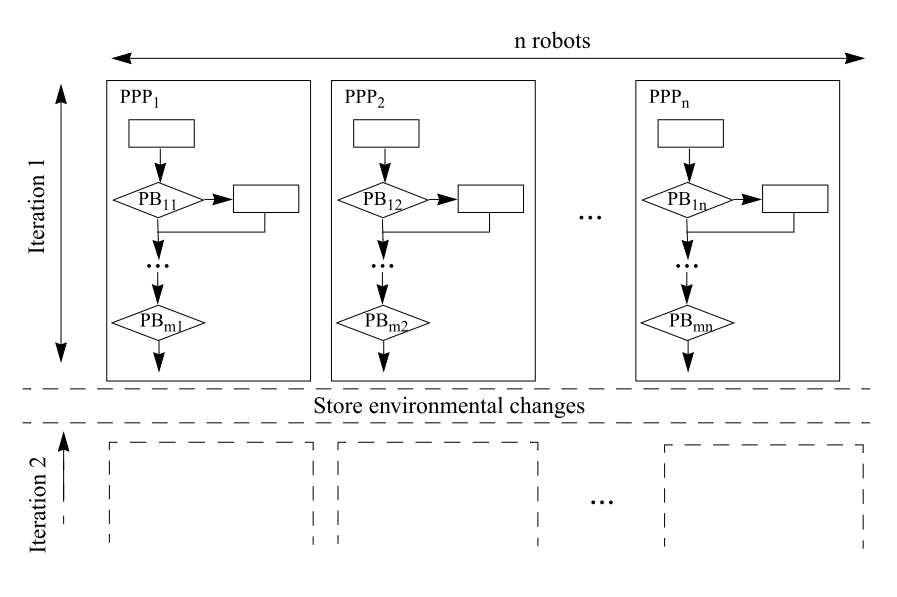
\includegraphics[width=15cm]{../assets/martinoliModelMethod.png}
\centering\caption{Gillespie simulation of a swarm system. Each controller, PPP$_i$, describes the independent behavior of a single robot in the swarm. Environmental variables are updated at the end of each iteration. (Image credit: Dr. Alcherio Martinoli)}\label{fig:micromodel}
\end{figure}

The Microscopic model (or micro-model) of a swarm system can be simulated using the \emph{Gillespie} simulation technique\cite{Gillespie1976,Gillespie1977}. Here, each agent is simulated individually using dice rolls and probability. Gillespie developed this simulation algorithm in the 1970s to model the time evolution of reactant and product volumes in a chemical reaction. The individual agents in his chemical system were single molecules of the reactant and the micro-model was derived from the dynamics of molecule interactions. The probability of two reactant molecules colliding was computed using simple physical properties such as the radius and velocity of the molecules in the reaction medium\cite{Gillespie1976}. Gillespie's original modeling approach has been modified for use with swarm systems, here. Martinoli outlines this process in detail in chapter 4.2 of his Ph.D. dissertation\cite{Martinoli1999b}. Robots with PFSM controllers are used instead of product and reactant molecules as the fundamental units of the simulation. First one step of the simulation, all robots are picked in a random order and their PFSMs are run in parallel for a single time-step. The state of the entire system is then updated and the process repeats itself for a pre-determined length of time. Unlike in the original version of Gillespie simulation where time-step lengths between reactions are also chosen at random, here we preset the length of time that passes between two steps of the simulation. 

\section{Verification of System Properties Using Real Experiments and Physics-Based Simulation}
\begin{figure}[!tb]
\begin{subfigure}{.5\textwidth}
\centering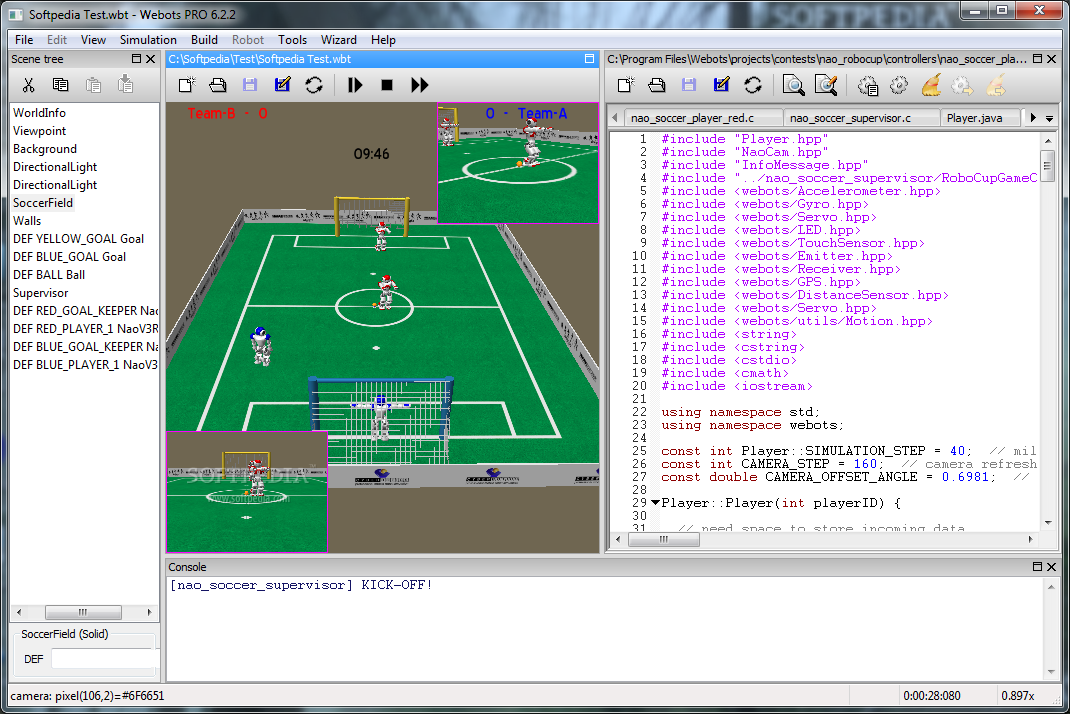
\includegraphics[width=6.5cm]{../assets/Webots.png}
\centering\caption{The Webots simulator rendering a game of robot soccer.}\label{fig:webots}
\end{subfigure}~
\begin{subfigure}{.5\textwidth}
\centering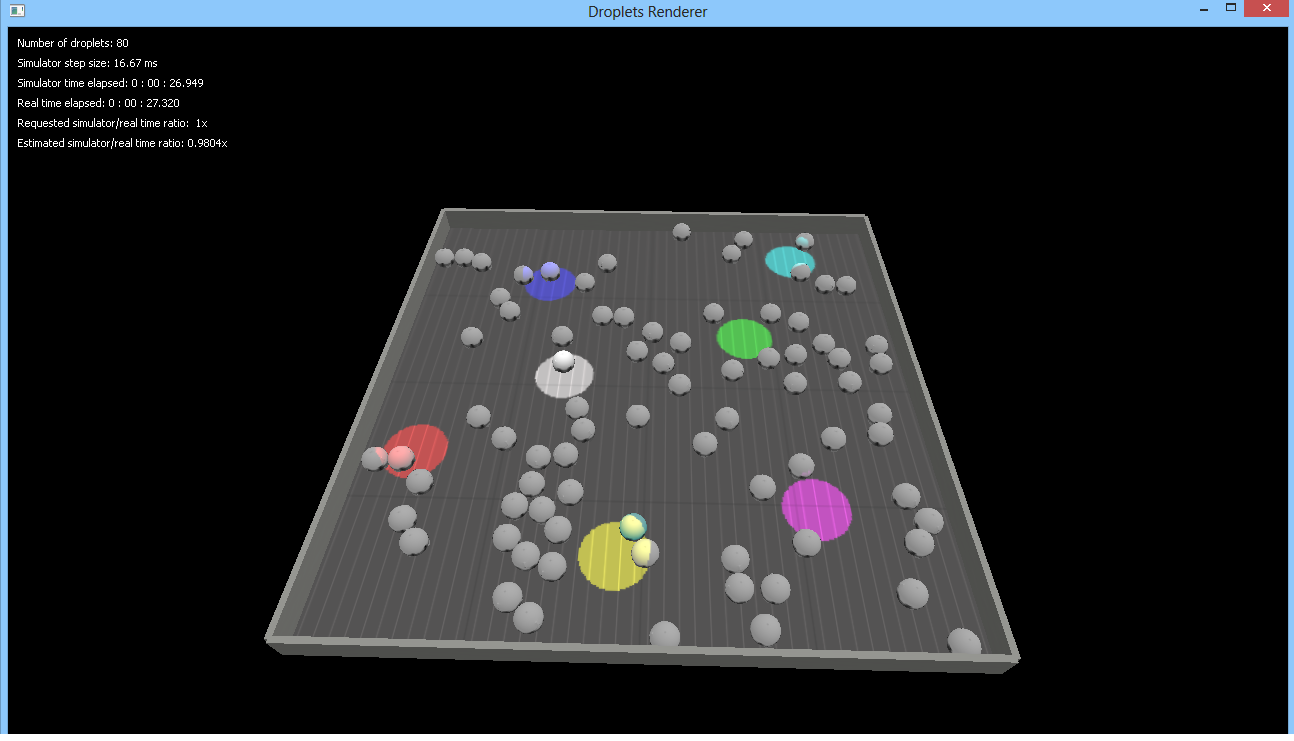
\includegraphics[width=6.5cm]{../assets/dsim.png}
\centering\caption{The Droplet swarm robot simulator}\label{fig:dropletsim}
\end{subfigure}
\caption{Swarm robot simulators.}
\end{figure}

An important step in any modeling process is validation by comparing model results to real experiment data. Given the relatively abstract approach applied so far for designing swarm robot models, this step is made even more crucial. The micro and macro-models in swarm robotics have conventionally been designed using observed phenomena from other processes seen in biological and chemical systems and adapted to fit the swarming task being studied. Many swarm algorithms show emergent behavior where the observation of complex properties at the system level cannot be trivially inferred from studying the individual agent behavior. The generalizations and simplifications made in the robot controller design when developing the micro and macro-models can, and in many cases do, suppress the interesting emergent properties seen in real physical systems. 

Physics-based simulators are often used to accurately recreate a task on a swarm system without investing the substantial time and resources required to develop and deploy real robots. These simulators attempt to remain as true to the real world as possible while maintaining an order of magnitude improvement in speed and simplicity over real robot experiments. Unlike micro-models that abstract away physical and environmental issues such as wheel slip, sensor noise, communication delays, etc., physics-based simulators make the added effort to accurately and dynamically model every minute aspect of the swarm system.

Many robot simulators are currently available today as either standalone programs like Webots (see Figure~\ref{fig:webots}). Webots is a widely used simulator in swarm robotics due to its capability to simulate multiple agents and agent-agent/agent-environment interactions in real time. The Webots API also allows for cross-compilation of programs from the simulation environment, right on to real robots without the need for reprogramming and supports a wide range of commercially available robot platforms such as Kilobots, Khepera, Alice, etc. There are also in-house implementations of physics simulators for specific robot platforms, such as the Droplet simulator shown in Figure~\ref{fig:dropletsim}, that build up on physics engines such as Bullet and ODE.

\section{Summary}
The different methods discussed in this section are widely used for modeling and analyzing multi-agent systems and their corresponding algorithms. Each modeling methodology provides advantages at different levels of abstraction:
\begin{enumerate}
	\item Gillespie simulation using FSM models allow us to study how micro-level individual agent interactions affect large scale behavior in the swarm.
	\item PFSM models and rate equations allow us to study the dynamics of the system which provides insight on macro-level aspects such as steady state analysis, parameter identification, equilibria, etc.
	\item Physics based simulations allow us to quickly verify our algorithms and provide a rapid prototyping tool for iterative refinement of swarm algorithms without having to invest in costly hardware.
\end{enumerate}

The following sections use at least a few of these methodologies to define and analyze new task-assignment strategies for multi-agent systems. In Chapter~\ref{ch:optimization} I use all of these methods and results from the following two chapters to propose a generalized framework for optimal control of a robot swarm.


%%%%%%%%%%%%%%%%%%%%%%%%%%%%%%%%%%%%%%%%%%%%%%%%%%%%%%%%%%%%%%%%%%%%%%%%%%%%%%%%
\chapter{Response Threshold Model for Multi-Agent Task-Assignment}\label{ch:resthmodel}
Drawing inspiration from TA in social insects, this chapter describes a novel approach to recruiting a variable number of agents for a particular task. Using CRT functions I show that the resulting macro-level agent team-size mean and variance can be controlled within desired ranges using only two micro-level parameters. Controlling variable team-sizes for TA in a MAS is an important step towards optimal control of the system as it uniquely identifies the important parameters involved in group size estimation of tasks of varying magnitude and difficulty. 

I consider a generic collaboration task with $m$ uniformly distributed collaboration sites within a flat arena with area $A$. A swarm of individually simple robots such as the \emph{Droplet} platform \cite{Farrow2014,Klingner2014} is deployed within the arena, uniformly and at random. The number of robots being used per experiment varies, as I discuss results for a number of different scenarios. Collaboration sites in the arena can be of various sizes and configurations.

Each individual agent is capable of locomotion \cite{Klingner2014} and local sensing \cite{Farrow2014}. The agents do not require global positioning and no centralized controller exists, but I assume each agent to be capable of local omnidirectional communication with other agents within its communication range. The agents are also capable of sensing the boundary of a collaboration site---I assume that sites have easily distinguishable boundary regions, as shown in Fig.~\ref{fig:dropletfire}, for the purposes of the model studied in this paper. 

The objective of each agent in the robot swarm is to find a collaboration site in the arena and perform a collective task with other agents at that site. The precise details of the collective task are not important for the purpose of understanding the coordination mechanism. I assume the actual collective task takes each agent a probabilistic finite amount of time to complete. Once collaboration is complete, the agent detaches itself from its current site and returns to searching for other sites in the arena. 

It is perfectly reasonable to assume that agents arrive at the same collaboration site after having just completed a task there (possibly unsuccessfully) but will now be part of a new collaboration group. Each agent individually decides whether or not to collaborate at a given time step, while waiting at a collaboration site. If the majority of agents at that site decide to collaborate then the entire population is recruited for the task and thus a collective consensus is reached using a majority voting scheme. Here, I consider a majority to mean exactly half or more of a given population. 

\begin{figure*}[!htb]
\centering\begin{subfigure}{.5\textwidth}
\centering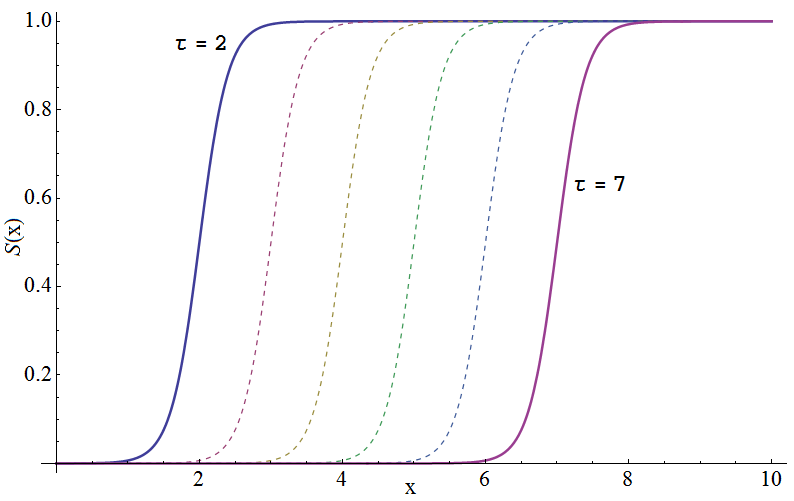
\includegraphics[width=\textwidth]{../assets/sigmoid2.png}
\caption{Changing $\tau$ offsets the curve along the $x$ axis, allowing to set the desired mean team size.}\label{}
\end{subfigure}~
\centering\begin{subfigure}{.5\textwidth}
\centering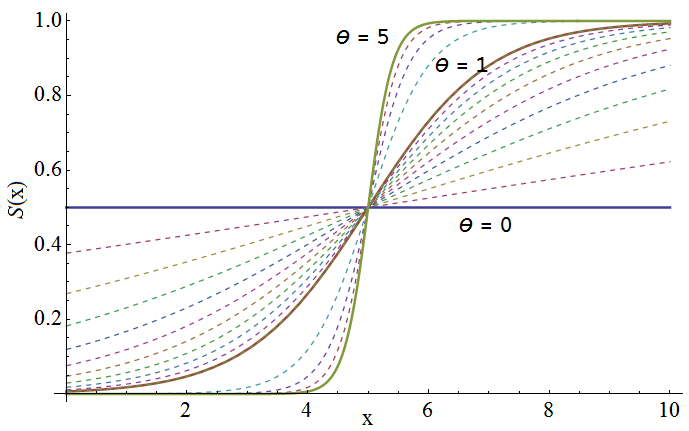
\includegraphics[width=\textwidth]{../assets/sigmoid1.png}
\caption{Changing $\theta$ changes the slope at the point $x^* = \tau$, $\sig(x^*) = 0.5$, allowing to control the team's variance.}\label{}
\end{subfigure}~
\caption{Sigmoidal response threshold function and its parameters.}\label{fig:sig}
\end{figure*}

An individual agent-$i$'s willingness to collaborate is a stochastic term governed by a sigmoid based RT function that takes as input, the number of agents $\xm$ currently at the same collaboration site as agent-$i$ and outputs a probability of collaboration using control parameters $\theta$ and $\tau$:
\begin{equation}
	\sig(\xm) = \frac{1}{1+e^{\theta(\tau - \xm)}}\label{eq:sig}
\end{equation}
The parameter $\theta$ controls the slope of the sigmoid function, while $\tau$ controls its offset along the $x$ axis, as seen in Fig.~\ref{fig:sig}. Each agent is independently responsible for estimating the group size $\xm$ at a given time either by direct sensing or by communication. In practice,  this involves building a list of unique identifiers of the agents sharing its collaboration site. The overall algorithm, followed by each individual agent in the system, is provided in Alg.~\ref{alg:sigalg}.

Note that the proposed response threshold function is different from \cite{Bonabeau1999}, who uses high-order polynomials. While these functions work well in regimes with moderate slope, they create numerical problems when approximating unit-step-like responses such as those (implicitly) used in \cite{Lerman2001}. I particularly chose the Logistic function from the large class of sigmoid functions due to the intuitive nature of the parameters $\tau$ and $\theta$. 

\begin{algorithm}
\caption{TA algorithm for an individual agent using the sigmoid threshold function}
\label{alg:sigalg}
\begin{algorithmic}
	\Function{Task\_Allocation}{$\theta$, $\tau$}
	\State $estimate \gets$ discover\_group\_size()
	\State $decision \gets$ run\_sigmoid($estimate$, $\theta$, $\tau$)
	\State communicate\_decision($decision$)
	\State $decisions[] \gets$ gather\_decisions()
	\State $result \gets$ Count($decisions[]$, $true$) \Comment{Count() Returns the number of successes in the decisions}
	\If{$result \geq (estimate / 2)$}
		\State Collaborate()
		\State \Return
	\Else
		\State Task\_Allocation($\theta$, $\tau$)
	\EndIf
	\EndFunction
\end{algorithmic} 
\end{algorithm}

\section{Macroscopic analysis}\label{sec:macromodel}
In this section I study how the local parameters $\tau$ and $\theta$ from an individual agent's sigmoid threshold function affect formation of groups of different sizes at the macroscopic system level.

Equation \eqref{eq:sig} is a cumulative probability density function approaching $1.0$ as the number of agents approaches infinity, that is $\lim_{x \to \infty}\sig(x)=1$. For $\theta \to \infty$, equation \eqref{eq:sig} approximates the unit step:
\begin{equation}
\lim_{\theta \to \infty} \frac{1}{1+e^{\theta(\tau-\xm)}}\approx
\left\{
\begin{array}{cc}
 1 & \hspace{.5cm} \xm>\tau \\
 1/2 & \hspace{.5cm} \xm=\tau \\
 0 & \hspace{.5cm} \xm<\tau
\end{array}
\right.\label{eq:siglim}
\end{equation}
Although, unlike the unit step function, the limit on the left in \eqref{eq:siglim} is always continuous, even at $\xm = \tau$ where the value of the sigmoid is $1/2$. The proposed model is therefore a generalization of the ``stick-pulling'' TA model with deterministic team size \cite{Lerman2001}, allowing us to tune the variable resulting group sizes using the tuning parameters $\tau$ and $\theta$ in \eqref{eq:sig}. 

Assuming the agents to be loosely synchronized, e.g., by considering decisions within a finite window of time, determining a majority vote corresponds to a Bernoulli trial with each agent flipping a biased coin---the bias being computed using the sigmoid function---to decide whether or not to collaborate in the next time step. The probability that exactly $k$ agents collaborate from a population of $n$ agents at a collaboration site is given by the probability mass function (PMF) of a Binomial distribution.
\begin{equation}
	B(n, k) = \binom{n}{k}\sig(n)^{k}\left(1 - \sig(n)\right)^{n - k}\label{eq:binomial}
\end{equation}

Since I care about the case when half or more of the agents ($n/2$) decide to collaborate, the probability $P(n)$ that half or more agents in a group of $n$ collaborate is the cumulative probability of the above PMF from $k = {n/2}$ to $k = n$. 
\begin{equation}
	P(n) = \sum\limits_{i={n/2}}^{n}\binom{n}{i}\sig(n)^{i}\left(1 - \sig(n)\right)^{n - i}\label{eq:cdf}
\end{equation}
This equation describes the probability with which a group of size $n$ at a given collaboration site will decide to successfully collaborate.  Note that \eqref{eq:cdf} is only an approximation for odd $n$, which requires rounding $\ceil{n/2}$ to the next integer. 

For large group sizes, the Binomial distribution approximates the Normal distribution and (\ref{eq:cdf}) reduces to 
\begin{equation}
P(n)=\int_{n/2}^{n} \mathcal{N}(n\sig(n),n\sig(n)(1-\sig(n)))\label{eq:normalcdf}
\end{equation}
Therefore, in a group of size $n$, and $n$ reasonably high (see below), an average of $n\sig(n)$ robots will collaborate with group sizes of variance $n\sig(n)(1-\sig(n))$. In the special case of $n=\tau$, i.e., the group size has the desired value of $\tau$, \eqref{eq:normalcdf} evaluates to $P(\tau) = \sig(\tau)=0.5$. Therefore, the probability of a group of $n$ agents to collaborate is identical to the probability of a individual agent to collaborate. In all other cases \eqref{eq:normalcdf} allows us to calculate the micro-macro matching from $\sig(n)$ to $P(n)$.  

A caveat of \eqref{eq:normalcdf} is that the Normal approximation yields poor results for small $n$, usually smaller than 20, and is better when $\sig(x)$ is neither close to 0 or 1 \cite{Box1978}. In these cases, exact solutions for $P(n)$ require numerical solutions of \eqref{eq:cdf} using what is known as \emph{continuity correction} \cite{Feller1945}. 

\section{Microscopic Model}\label{sec:micromodel}
As the proposed collaboration mechanism are strongly non-linear, I chose microscopic stochastic simulations to explore the underlying dynamics of the system. The approach followed to build the stochastic Gillespie simulation of the system is as follows.
\begin{itemize}
\item Perform random walk till a collaboration site is found (\emph{search} state).
\item Perform algorithm, Task\_Allocation (see Algorithm \ref{alg:sigalg}) (\emph{wait} state).
\item Complete collective task and disperse. (\emph{collaborate} state).
\item Return to search.
\end{itemize}

The probabilistic finite state machine that describes individual agent behavior for this swarm system is shown in Fig.~\ref{fig:sm}. From the individual agent's perspective only one state each exists for \emph{wait} and \emph{collaborate}. From a probabilistic modeling perspective, the wait and collaborate states are meta states, divided into $m$ states each, one for each collaboration site in the arena. This is done to clarify that the probability of collaborating at a given site \emph{only} depends on the number of agents at that specific site and collaborations \emph{only} happen between agents at the same site.

The probability $p_{SW_i}$ in the PFSM model of the system shown in Fig.~\ref{fig:sm} is the probability that an agent encounters a collaboration site. This is geometrically computed as the ratio between the total area of the search space (arena) and the total area of collaboration sites, i.e. $p_{SW_i} = n_s(A_s)/A$ ($n_s$ = number of sites, $A_s$ = area per site). The probability, $P_{W_iC_i}$, of going from a wait state to a collaboration state is given by eq.~\eqref{eq:cdf} with input $N_{W_i}$, the number of agents at collaboration site-$i$. $P_{C_iS}$ stochastically models the time it takes for an agent to complete a generic collaborative task and is equal to $1/T$, where $T$ is the amount of time (on average) that it takes an agent to complete the collective task. Note that agents have a zero probability of transitioning from the \emph{wait} state back to the \emph{search} without collaborating, i.e. once an agent is at a collaboration site, it will not leave till a collaboration event happens at that site. I chose the following numerical values for all simulations, unless otherwise noted: $A=100cm^2$ and $A_s=10cm^2$.

For the sake of simplicity, consensus between agents---i.e. going from $W_i$ to $C_i$---at the same collaboration site is assumed to happen instantly and therefore the extra state(s) is/are omitted from robot controller.
\begin{figure}[!htb]
	\centering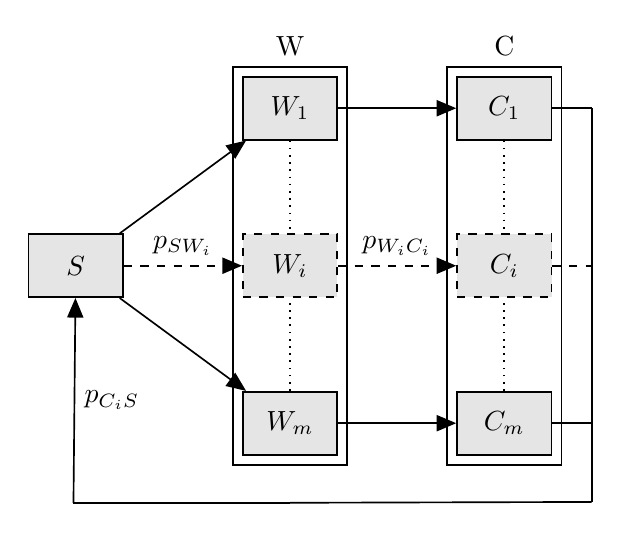
\begin{tikzpicture}[->,>=triangle 45,auto,node distance=2cm, semithick,
		state node/.style={rectangle, draw, fill=black!10, minimum height=.8cm, minimum width=1.2cm},
		meta node/.style={rectangle, draw},
		dashed node/.style={rectangle, draw, dashed, fill=black!10, minimum height=.8cm, minimum width=1.2cm}]

 	\node[state node] (1) {$S$};
 	\node[dashed node] (2) [right = 1.5cm of 1] {$W_i$};
 	\node[state node] (3) [above of=2] {$W_1$};
 	\node[state node] (4) [below of=2] {$W_m$};
 	\node[meta node, fit={(2) (3) (4)},label=above:{W}] {};
 	\node[dashed node] (5) [right = 1.5cm of 2] {$C_i$};
 	\node[state node] (6) [above of=5] {$C_1$};
 	\node[state node] (7) [below of=5] {$C_m$};
 	\node[meta node, fit={(5) (6) (7)}, label=above:{C}] {};
 	\coordinate[right=0.5cm of 6] (8);
 	\coordinate[right=0.5cm of 6] (8);
 	\coordinate[right=0.5cm of 6] (8);
 	\coordinate[right=0.5cm of 6] (8); 	 	
 	\coordinate[below of=8] (9);
 	\coordinate[below of=9] (10);
 	\coordinate[below= 1cm of 10] (11); 
 	\coordinate[below= 0.6cm of 4] (12);
 	\coordinate[left= 2.75cm of 12] (13);

		\path	(1) 	edge[dashed] node{$p_{SW_i}$} (2)
						edge[] node{} (3)
						edge[] node{} (4);
		\path	(2) 	edge[dashed] node{$p_{W_iC_i}$} (5);
		\path	(3) 	edge[] node{} (6)
						edge[-,dotted] node{} (2);		
		\path	(4) 	edge[] node{} (7)
						edge[-,dotted] node{} (2);		
		\path	(5) 	edge[-, dashed] node{} (9);
		\path	(6) 	edge[-] node{} (8)
						edge[-, dotted] node{} (5);
		\path	(7) 	edge[-, dotted] node{} (5)		
						edge[-] node{} (10);		
		\path	(8) 	edge[-] node{} (9);
		\path	(9) 	edge[-] node{} (10);
		\path	(10) 	edge[-] node{} (11);
		\path	(11) 	edge[-] node{} (12);
		\path	(12) 	edge[-] node{} (13);
		\path	(13) 	edge[] node[right= 0cm of 13]{$p_{C_iS}$} (1);
\end{tikzpicture}
\caption{Agent controller used to drive group collaboration. There is a Search state and $m$ Wait and Collaboration states, $W_i$ and $C_i$ respectively---one for each collaboration site.}\label{fig:sm}
\end{figure}

In order to compare the dynamics of the proposed probabilistic TA mechanism with the deterministic one by Lerman et. al\cite{Lerman2001}, I implemented a variation of the above algorithm using a unit-step at $\tau$ instead of the sigmoid function and removing the consensus step, which is not necessary in this model. 

I use Gillespie simulation \cite{Gillespie1976} to explore the dynamics of the proposed collaboration model.
For both experiments a single collaboration site is used and each run simulates 300s of time. The desired group size ($\tau$, in Eq.~\eqref{eq:sig}) is set to 4, 8, 16 and 32 agents out of a total of 100 robots. The collaboration task is programmed to take 10s, on average, per agent. Data points are gathered by averaging data from 100 identically set up runs in each case. The \emph{rate of collaboration} for the threshold model is computed by summing the number of groups that successfully collaborate and dividing by the total experiment time (300s). For the deterministic model, collaboration rate is computed by summing all successful collaborations, i.e. collaborations involving team sizes equal to $\tau$, and dividing the the experiment time (300s).

\section{Experiments and Results}
\begin{figure*}[!htb]
\begin{subfigure}{0.33\textwidth}
\centering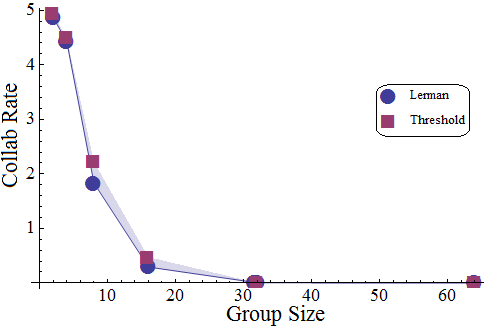
\includegraphics[width=1.0\textwidth]{../assets/LermanCollabCompare3.png}
\centering\caption{$\theta=2$}\label{fig:lercol3}
\end{subfigure}~
\begin{subfigure}{0.33\textwidth}
\centering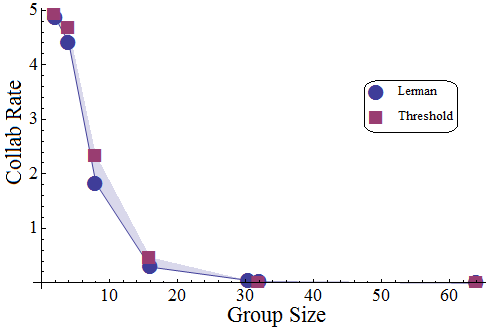
\includegraphics[width=1.0\textwidth]{../assets/LermanCollabCompare2.png}
\centering\caption{$\theta=1$}\label{fig:lercol2}
\end{subfigure}~
\begin{subfigure}{0.33\textwidth}
\centering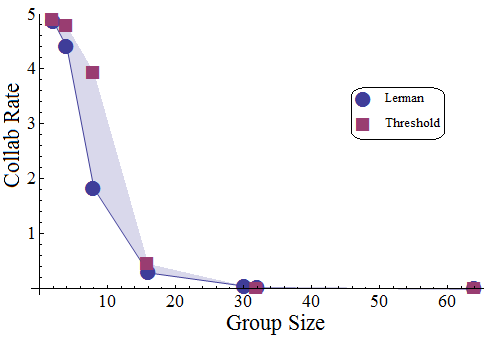
\includegraphics[width=1.0\textwidth]{../assets/LermanCollabCompare1.png}
\centering\caption{$\theta=0$}\label{fig:lercol1}
\end{subfigure}
\caption{Comparison of the collaboration rate for TA with probabilistic and deterministic \cite{Lerman2001} for different values of $\theta$ and team sizes $\tau$ in an environment with one collaboration site and one hundred robots. }\label{fig:lercol}
\end{figure*}

I will first compare the dynamics of the proposed approach with Lerman et al.'s k-collaboration model \cite{Lerman2001} and then validate the emergence of group sizes with similar means but varying variances.

Figure \ref{fig:lercol3} shows collaboration rates for both models when $\theta$ is set to 2 (for the probabilistic model) and the wait time is set to $\infty$ (for the deterministic model), in order to allow for a fair comparison. (All experiments are run in a regime where infinite wait times are optimal wait times, i.e., there are more agents than collaboration sites.) Figures \ref{fig:lercol3}, \ref{fig:lercol2} and \ref{fig:lercol1} show collaboration rates for $\theta = 2$, $\theta = 1$ and $\theta=0$ with infinite wait time. With $\theta=0$, the Logistic function is uniformly 0.5, allowing any team size to form.  
With increasing $\theta$ the Logistic function approximates a unit step, minimizing the variance. 

\begin{figure*}[!htb]
\begin{subfigure}{0.5\textwidth}
\centering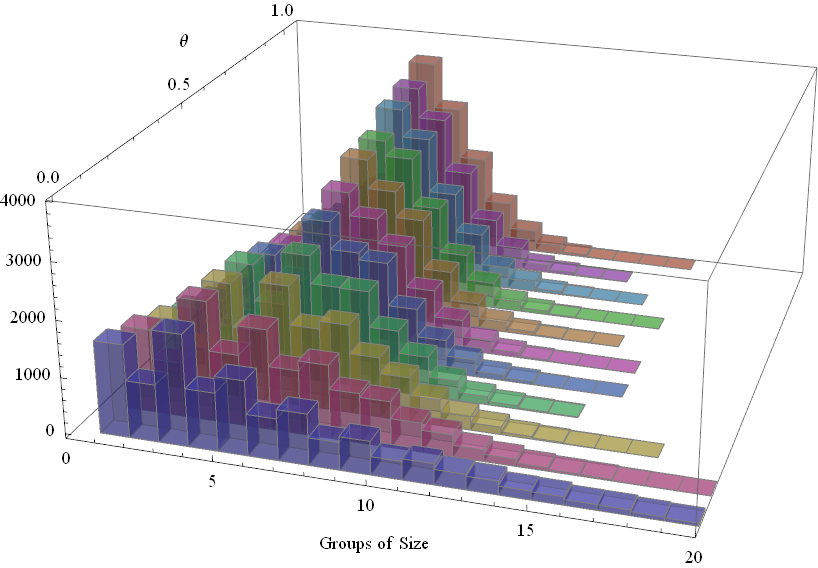
\includegraphics[width=1.0\textwidth]{../assets/collabratesweep4.png}
\centering\caption{$\tau = 4$}\label{fig:collabsweep4}
\end{subfigure}~
\begin{subfigure}{0.5\textwidth}
\centering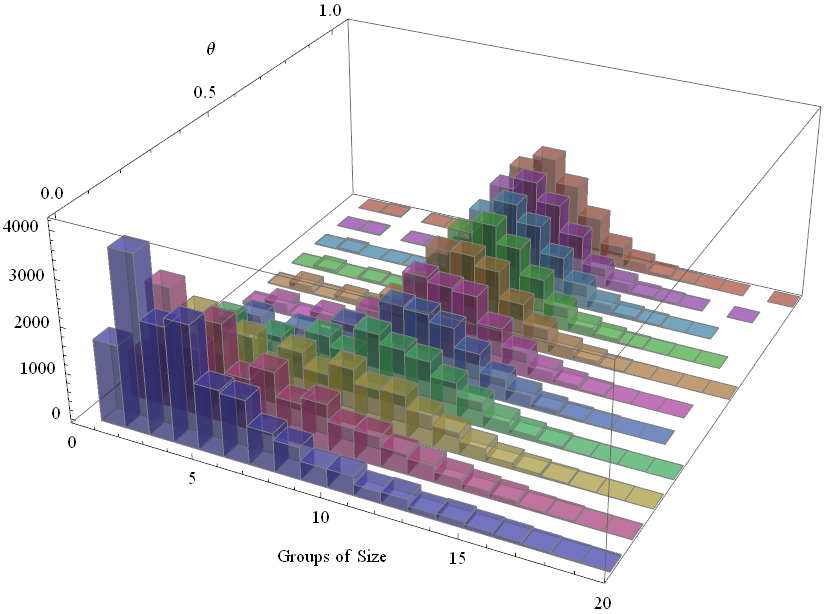
\includegraphics[width=1.0\textwidth]{../assets/collabratesweep8.png}
\centering\caption{$\tau = 8$}\label{fig:collabsweep8}
\end{subfigure}
\begin{subfigure}{0.5\textwidth}
\centering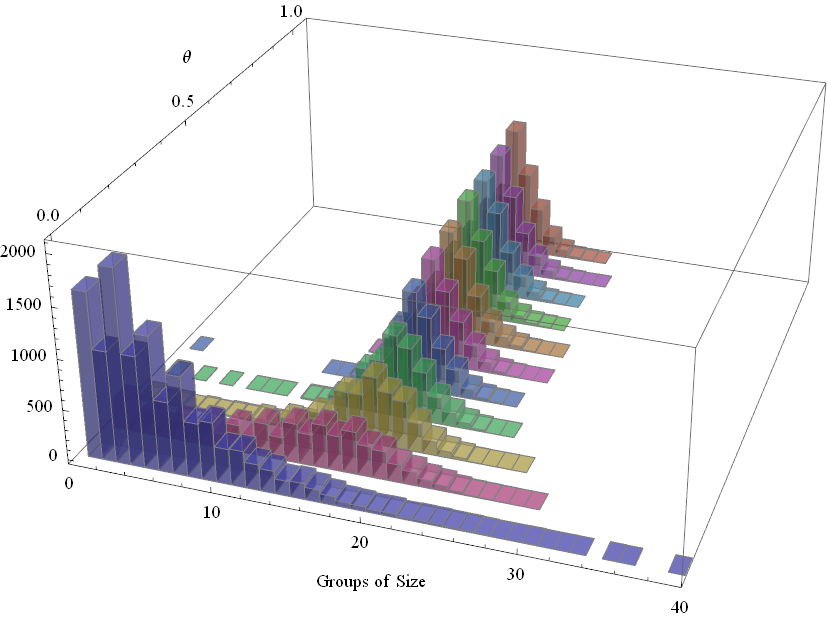
\includegraphics[width=1.0\textwidth]{../assets/collabratesweep16.png}
\centering\caption{$\tau = 16$}\label{fig:collabsweep16}
\end{subfigure}~
\begin{subfigure}{0.5\textwidth}
\centering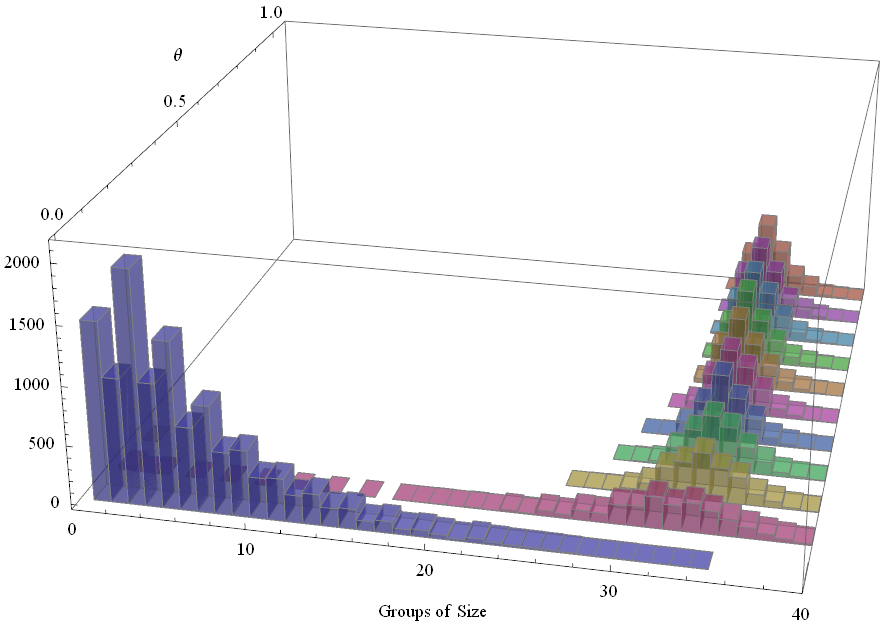
\includegraphics[width=1.0\textwidth]{../assets/collabratesweep32.png}
\centering\caption{$\tau = 32$}\label{fig:collabsweep32}
\end{subfigure}
\caption{Histograms of resulting team sizes for various values of $\tau$ and $\theta$ with one hundred robots and one collaboration site.}\label{fig:collabsweep}
\end{figure*}

I observe the collaboration rate to be qualitatively and quantitatively very similar for high values of $\theta$ (steep slope), and to exceed that of the deterministic model for very low values of $\theta$ (flat slope). This is expected as flat slopes increase the variance of the observed group size and therefore allow much smaller teams than $\tau$ agents to collaborate.

\begin{figure}[!htb]
\begin{subfigure}{0.5\textwidth}
\centering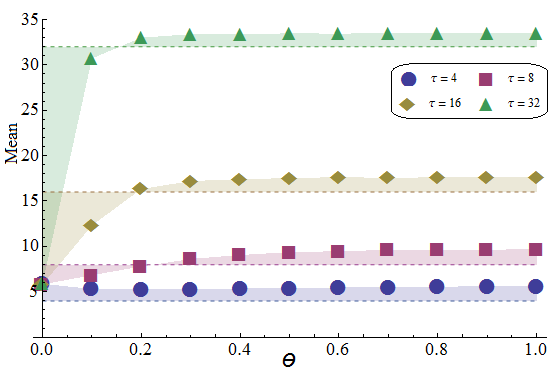
\includegraphics[width=1.0\textwidth]{../assets/means.png}
\centering\caption{}\label{fig:means}
\end{subfigure}~
\begin{subfigure}{0.5\textwidth}
\centering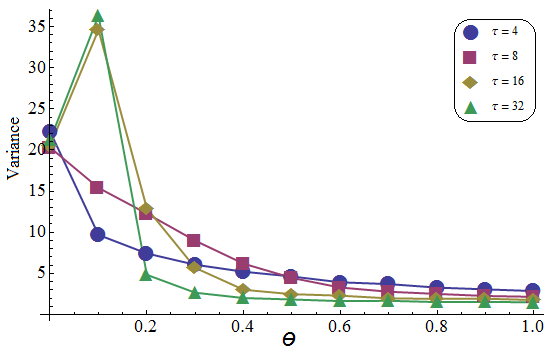
\includegraphics[width=1.0\textwidth]{../assets/variances.png}
\centering\caption{}\label{fig:vars}
\end{subfigure}
\caption{Showing the effects of varying $\theta$ on means and variances corresponding to the histograms seen in Fig.~\ref{fig:collabsweep}.}\label{fig:meansvars}
\end{figure}

Figure \ref{fig:collabsweep} shows histograms of the resulting group sizes for various values of $\tau=4, 8, 16, 32$ and $\theta=[0;0.1;1]$ (100 simulations per data point). It is clearly seen that when $\theta$ is set to 0, the sigmoid becomes constant ($\sig(x) = 1/(1 + e^{0}) = 0.5$) so agents have an equal probability to want to collaborate or not, no matter what the desired group size is. I therefore see a large number of small groups forming, with most groups consisting of 2 agents. This is to be expected since the expected number of agents willing to collaborate in a group of size 2 is 1, given the probability of collaboration is constant at 0.5.

Figure \ref{fig:means} displays average group sizes as $\theta$ is varied from 0 to 1 and $\tau$ from 4 to 32 based on the data from Figure \ref{fig:collabsweep}. I observe that for large enough values of $\theta$ the mean of the group size distribution approaches the desired group size and is largely unaffected by increasing $\theta$. Thereafter, its magnitude depends only on $\tau$ except in the special case where $\theta = 0$ where it is constant. The relative error of the mean compared to the desired average decreases with increasing number of agents as the  Binomial distribution \eqref{eq:cdf}
approximates the Normal distribution \eqref{eq:normalcdf}.

Figure \ref{fig:vars} shows how the variance of group size decreases with increasing $\theta$. This is because the sigmoid function approximates the unit step, making the team size more and more deterministic. On the other hand, low values of $\theta$ lead to large variances in the group size. For $\theta=0$, the variance is constant for all values of $\tau$ and depends exclusively on the total number of robots. 

Finally, I use the Droplet swarm robot platform to perform real experiments to study the effects of using the proposed TA scheme on a physical system. The Droplets are small individually simple robots capable of omni-directional motion and communication (via IR) as well as sensing patterns projected from above. In my experiment I assume that all agents have already arrived at a collaboration site and measure the corresponding collaboration rates for a team of 6 robots while varying values of $\tau$ and $\theta$. Each agent is individually running the algorithm described in Alg.\ref{alg:sigalg}. A collaboration event is recognized by having all the robots turn on their green LEDs for 5 seconds. After such a collaboration event, each agent resets its group size estimate and runs Alg.\ref{alg:sigalg} again. 

\begin{figure}[!htb]
\centering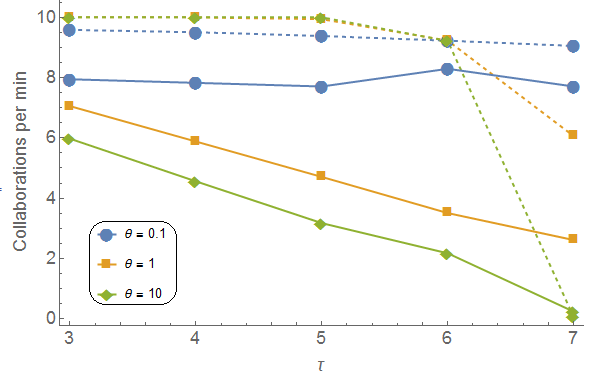
\includegraphics[width=0.55\textwidth]{../assets/realsimexpnew.png}
\caption{The solid lines show collaborations per min, over 15min, for a group of 6 real robots as the desired group size is varied from 3 to 7 and the slope of $\sig$ is varied between $0.1, 1$ and $10$. The dashed lines indicate simulation results with the same parameters.\label{fig:expdat} }
\end{figure}

I ran $5$ repeated experiments for all $15$ combinations of $\tau = 3,4,5,6$ and $7$, and $\theta = 0.1, 1$ and $10$, totally $75$ runs. Each experiment lasted 15 minutes and an overhead camera system was set up to detect collaboration events using the software \emph{RoboRealm}. The collaboration rate was a value computed by counting the number of collaborations over the course of each 15 minute experiment, normalizing to collaborations per minute, and averaging over the 5 repeated runs. 
To account for the vision software's detection errors, the raw data gathered from each experiment was de-bounced and passed through a low-pass filter to expose real collaboration events while eliminating observation error. The results of these experiments are seen in Figure \ref{fig:expdat}. While results are in accordance with simulation for $\theta$ being low, the collaboration rate on the real robot platform is much lower than expected for larger $\theta$ as simulation assumes perfect communication and group size estimates.


%%%%%%%%%%%%%%%%%%%%%%%%%%%%%%%%%%%%%%%%%%%%%%%%%%%%%%%%%%%%%%%%%%%%%%%%%%%%%%%%
\section{Discussion}
Results in Figures \ref{fig:lercol}, \ref{fig:collabsweep} and \ref{fig:meansvars} show that the proposed threshold-based TA mechanism is a generalization of the deterministic Lerman model in that it allows to approach what is seen with deterministic group sizes while retaining the elasticity to vary group sizes along any desired range of values. Also, these plots show how altering microscopic control parameters within the agents, $\theta$ and $\tau$ of their sigmoid functions, directly affects macroscopic behavior of the swarm system by altering means and variances of formed group sizes, respectively. Although the matching between microscopic results and macroscopic prediction is not perfect due to the discrete approximation, the plots show that a wide range of means and variances are feasible. Finding appropriate parameters to reach these could be easily achieved using a suitable optimization framework such as presented in \cite{Correll2008,Berman2009}, using the macroscopic predictions as initial estimate. 

The proposed TA algorithm requires an estimate of the group size at each collaboration site as well as the ability to communicate with the group in order to reach a consensus. While these assumptions seem to be limiting at first sight, they can be rolled into the analysis process and possibly exploited to design the TA process. For example, an increasing variance for observing the group size $\tau$ or noise in the consensus process simply increase the variance of the TA process and could therefore be countered---to some extent---by altering the properties of the response threshold function. 

This effect is clearly observed in the physical experiment results (see Figure \ref{fig:expdat}). Since the communication between real robots is not perfect, they almost always  underestimate the size of their group resulting in lower collaborations for high $\theta$ and $\tau$ values. As I observe from comparing the micro simulation results---that are modeled with perfect communication---with real experiment data, I observe a large discrepancy when $\theta = 10$. This happens because although individual agents are set up to be in a group of size 6, their estimates for the group size never cross 4 due to imperfect and blocked communication. Coupled with the fact that the sigmoid threshold effectively acts as a step function when $\theta = 10$, this results in approx. 0 probability of collaboration between agents for a desired group size of 6 but a group size estimate of $\leq 4$. Lower values of $\theta$ result in better matching between real and simulation data since lower slopes effectively increase the variance in allowed group sizes and mitigate this effect.

I note that there is no optimal wait time as in stick pulling-like collaboration \cite{Lerman2001}. This optimum exists in swarms with less robots than sticks, which is shown analytically in \cite{Martinoli2004}. Such an optimum does not exist in the proposed model as there is a non-zero probability team sizes with $n<\tau$ will eventually collaborate. Indeed, Algorithm \ref{alg:sigalg} eventually completes as $\sig(x) > 0 \forall x$, i.e., even if only very few robots are at a collaboration site and $\tau$ is large, there is a non-zero probability that half or more of the agents at the site eventually collaborate (see also Equation \ref{eq:cdf}).

Although the algorithm does not deadlock---the probability to collaborate even if the team size is far off the desired value---the resulting behavior might be undesirable, resulting in potentially very long wait times and poor task performance. This could be mitigated by introducing preferential detachment from small groups and preferential attachment to larger groups as customary in swarm robotic aggregation \cite{Correll2011}.

In practice, effective collaboration rates will also be limited by the embodiment of the robots, which might make finding physical space at a site cumbersome. In the presented microscopic simulation, for both stochastic and deterministic team sizes, the number of robots per site were not limited, allowing scenarios in which multiple groups collaborate in quick succession at the same site. While comparing both models without embodiment is reasonable, I wish to study the effect of embodiment in future work.

\section{Summary}
In this chapter I presented a multi-agent collaboration algorithm to recruit an approximate number of individually simple robots with controllable variance. I proposed a sigmoid RT function motivated by TA in social insects and describe macro-level models backed by micro-level simulations to predict the resulting team sizes and their variance.  These results were further validated through physical experiments using the \emph{Droplet} swarm robotics platform. I showed that the slope of the response threshold function could be used to control the variance of group size, allowing agents to trade off deterministic team size with coordination speed, and making the proposed mechanism applicable to a variety of applications.

%%%%%%%%%%%%%%%%%%%%%%%%%%%%%%%%%%%%%%%%%%%%%%%%%%%%%%%%%%%%%%%%%%%%%%%%%%%%%%%%
\chapter{Existence of an Equilibrium Strategy for Communication-Free Multi-Robot Task-Assignment}\label{ch:existeqrtm}
A number of different methods exist for TA in MAS such as deterministic leader-follower coalition algorithms \cite{Chen2011} and more complex market-based approaches \cite{Amstutz2008} to simpler probabilistic algorithms for individually simplistic agents \cite{Dantu2012}. As mentioned earlier, the reason that I focus so heavily on the RT model is it's widespread use in ethology research for modeling social insects. While this phenomenological evidence provides a solid incentive for their use in engineered robotic systems, there has so far been no mathematical argument for their use. In this chapter I provide---for what I believe to be the first time in the field of swarm robotics---a mathematical explanation for their prevalence using a well known result from game theory\footnote{I would like to thank Dr. Behrouz Touri for his extensive help on the theory of global games and in formulating and proving the theorems mentioned in this chapter.}. The problem of TA in MAS is formulated as a global game and two theorems are subsequently proved showing the existence of a Bayes Nash Equilibrium in a system using DRTs (Theorem 1) and, subsequently, CRTs (Theorem 2) for TA in MAS. Theorem 2 also analytically shows how Gaussian noise in perceiving stimulus signals leads to sigmoid RTs, as are commonly observed in nature.

\section{Global Games: A Brief Overview}\label{sec:ggoverview}
Game theory is the study of strategic interactions among multiple agents or players, such as robots, people, firms, etc.\~where the decision of each party affects the payoff of the rest. A fundamentally important class of games is one with incomplete or imperfect information where each agent's utility depend not only on the actions of the other agents, but also on an underlying fundamental signal that cannot be accurately ordained by the agents. The class of global games with incomplete information was originally introduced in \cite{Carlsson1993} where two players are playing a game and the utility of the two players depends on an underlying fundamental signal $\tau \in \mathbb{R}$, but each agent observes a noisy variation of this signal, $x_i$. Returning to my previous example of firefighting (as seen in Figure~\ref{fig:ggsetup}), this fundamental signal $\tau$ is the \emph{magnitude} of the task of putting out the fire, i.e., the number of robots needed to do so. The size and intensity of the fire, along with environmental and other site-specific factors all play a major role in determining whether an agent should begin the task or wait for more help to arrive.

While I use the term magnitude to describe $\tau$, it is a stand-in for a simplified representation of a more abstract quality of any task. All tasks demand completion and the act of completion requires resources, be it time and/or energy of some form. In swarms of minimalist agents with limited capabilities, the resource required to collaboratively complete a task is invariably quantized into the number of agents attempting to complete that task. In bee hives and ant colonies the drive to complete a task is regulated by pheromone levels, among other signals.  In engineered swarm systems, more direct measurements of the environment through the use of on-board sensors allow a robot to independently estimate $\tau$, however imperfectly. In either case, $\tau$ is an inherent \emph{truth} about the task that can never be discerned accurately, but is always indirectly estimated by all agents. It is important to highlight that agents never share their independent estimates of $\tau$ with each other in my proposed formulation of the TA problem. While this may seem like a weakness in my argument, most of the research on RT TA explicitly mentions limited to no communication requirements to be a major advantage of this approach versus other methods since even limited information propagation through a $>1000$ agent system quickly becomes the bottleneck for any distributed swarm algorithm.

\section{Concurrent Benefit Task with Imperfect Information}\label{sec:conbenefit}
In this section, I mathematically define a \emph{concurrent benefit} task which is central to my study. Informally, concurrent benefit is an attribute of a collaborative task where a certain minimum number of agents is needed to solve a task; if this number is not reached, agents which try nevertheless waste their efforts. In addition, the exact number of agents required to successfully complete the task is unknown and varies over time due to numerous, complex physical parameters. Many collaborative tasks---particularly those seen in biological systems---exhibit the property of concurrent benefit ranging from surveillance and coordinated defense of enclosed areas like termite mounds and honey bee hives \cite{Breed1990} to collective transport of heavy objects and even containment of oil spills and forest fires. The probability of success depends, non-linearly, on the average number of agents assigned to that task. For example, 5--10 ants may be insufficient to lift a heavy object such as a small rock or twig and will waste a considerable amount of energy and time in trying, but 12 or more ants might accomplish the task successfully. Similarly, in a MAS setting, consider the task of collaborative firefighting. To contain a large fire, it is insufficient (and inefficient) for a single agent to start putting out the fire without waiting for backup. But the rate of fire containment increases quickly by adding just a few more agents to the group, which illustrates the property of concurrent benefit well. The proofs presented in this chapter relates to this aforementioned class of collaborative tasks.

\subsection{Formal Definition of a Concurrent Benefit Task}\label{subsec:conbenefitdef}
Consider a set of $n$ robots and suppose that each robot has an action set $A_i=\{0,1\}$ where $0$ represents not participating in the task and $1$ represents participating in the task. Every agent is also aware of the total number of other robots, $n$ in the system. The decision to act or not act is made by all agents at the same time, i.e. this is a one-shot game with no notion of time. The magnitude parameter $\tau$ of the given task also plays an important role in my formalism. I let $\tau$ be an (often random) real number which represents how many agents are required to complete a task. I further assume that it belongs to an interval $E=[c,d]$ in $\R$.  Finally, I let $u_i:A_i\times\Z^+\times \R\to \R$ be the utility of the $i^{\text{th}}$ robot, where $u_i(a_i,g,\tau)$ is the utility of the $i^{\text{th}}$ robot when $g$ other robots have decided to participate in the task of magnitude $\tau$\footnote{In general, the utility of each robot depends on the joint actions of the rest of the robots. However, here I assume that the utility depends only on the number of robots participating in the activity. The following discussions can be substantially generalized to a more general setting but this form of utility serves the purpose of this study.}.\\
I define a task $T$ to be a \emph{concurrent benefit task} if:
\begin{enumerate}[a.]
	\item $u_i(1,g,\tau)-u_i(0,g,\tau)$ is an increasing and continuous function of $\tau$ for any $a_i\in A_i$ and $g$. I further assume that $|u_i(1,g,\tau)-u_i(0,g,\tau)|\leq \tau^p$ for some $p\geq 1$. 
	\item For extreme magnitude ranges, taking part in the activity is either appealing or repelling, i.e.\ there exists $\underline{\tau},\bar{\tau}\in (c,d)$ with $\underline{\tau}\leq \bar{\tau}$ such that for any $\tau\geq \bar{\tau}$, I have $u_i(1,g,\tau)>u_i(0,g,\tau)$ and for $\tau\leq \underline{\tau}$, the only equilibrium of the game is $(0,0,\ldots,0)$. 
\end{enumerate}

Note that in order to have such a task, I need the above conditions to hold for all the robots, i.e.\ for all $i\in\{1,\ldots,n\}$.
An example of a utility function that would satisfy such conditions is a function $u_i(a_i,g,\tau)=a_i(1-e^{-(g+1)}+\tau)$. Also, note that in a typical robotics scenario, the robots have a common utility function which is aligned with the system's objective. But in general, they may have different utility functions that need to satisfy the above conditions. 

\begin{figure}[!htb]
\centering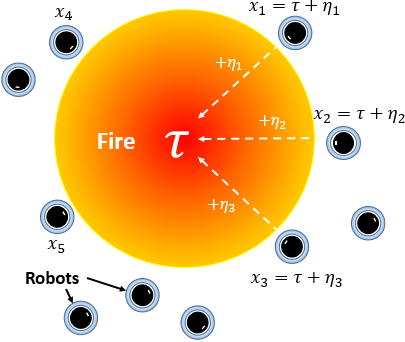
\includegraphics[width=0.65\columnwidth]{../assets/globalgamesetup.png}
\centering\caption{A multi-robot firefighting scenario set up as a global game. Each player's imperfect estimate of the task is represented by $x_i$, a sum of the global magnitude parameter-$\tau$ and noisy sensor measurements-$\eta_i$.}\vspace{-10px}\label{fig:ggsetup}
\end{figure}

The main challenge in devising strategies in performing a concurrent benefit task is that the knowledge of the magnitude parameter is not easily accessible to the robots. For example, consider the firefighting scenario described earlier. The magnitude of the task is not easily estimated by each robot and they only have noisy, imperfect information through their on-board sensors and their local measurements.  I model this imperfect knowledge by assuming that robot $i$ observes $x_i=\tau+\eta_i$ where $\eta_i$ is a Gaussian $\mathcal{N}(0,\sigma_i^2)$ random variable, as seen in Fig.~\ref{fig:ggsetup}. Throughout my discussion, I assume that the task magnitude $\tau$ is a Gaussian random variable\footnote{This analysis is extendable to a larger class of random variables but for the simplicity of the discussion, I consider Gaussian random variables here.} and it is independent of $\eta_1,\ldots,\eta_n$. Now, the main question is that given a robot's private measurement $x_i$, what is a \emph{sensible strategy} to follow?

I refer to a function that maps measurements (observations) to actions $A_i$ as a \emph{strategy}. Mathematically, a strategy $s_i$ for the $i$th robot is a (measurable) function $s_i:\R\to A_i$. Strategy $s_i$ prescribes what action the $i$th robot should take given its own measurement $x_i$. Given this, consider a set of robots with strategies $s_1,\ldots,s_n$. Let us denote the strategies of the $n-1$ robots other than the $i$th robot by the vector $s_{-i}=(s_1,\ldots,s_{i-1},s_{i+1},\ldots,s_n)$.  I say that a strategy $s_i$ is a \emph{threshold strategy} if $s_i(x)=\text{step}(x, t_i)$, i.e.\ the step function with a jump from 0 to 1 at $t_i$. For the $i$th robot, I define the best-response $BR(s_{-i})$ (to the strategies of the other robots) to be a strategy $\tilde{s}$ that for any $x\in \R$:
\begin{align*}\label{eqn:BR}
BR(s_{-i})(x)&=\tilde{s}(x)=\amax{a_i\in A_i} E(u_i(a_i,g,\tau)\mid x_i=x)\\
&=\amax{a_i\in A_i} E(u_i(a_i,\sum_{j\not=i}s_j(x_j),\tau)\mid x_i=x),
\end{align*}
where $E(\cdot \mid x_i)$ is the conditional probability of $u_i$ given the $i$th agent's observation. Note that given $x_i$ and the strategies of the other robots $s_{-i}=(s_1,s_2,\ldots,s_{i-1},s_{i+1},\ldots,s_n)$, $\tau$, and $s_j(x_j)$ will be a random variable. In other words, given the $i$th robot's observation $x_i$, the observation of the other robots and hence, their actions would be random from the $i$th robot perspective.

Now, to define a \emph{sensible strategy} I say that a strategy profile $s=(s_1,\ldots,s_n)$ is sensible strategy if it leads to a \emph{Bayesian Nash Equilibrium} (BNE) \cite{Fudenberg1998}, given $s_i=BR(s_{-i})$ $\forall i\in \{1,\ldots,n\}$. In other words, with the current strategies of the $n$ robots, no robot has the incentive to deviate from its current strategy.

\subsection{Threshold-Based Bayesian Nash Equilibrium}\label{subsec:thmproof}
I now show that any task with concurrent benefit admits a threshold strategy BNE. In other words, it is sufficient for the agents to follow a simple algorithm: 
\begin{enumerate}[(i)]
\item Compare your noisy measurement $x_i$ to a threshold value $\td_i$,
\item If the measurement is above $\td_i$ take part in the collaborative task, otherwise hold off. 
\end{enumerate}

In general, the existence of a BNE for a game is a questionable fact, especially once additional constraints are imposed on the structure of strategies. However, in this case, I can show that there exists a sensible threshold policy for the class of tasks with concurrent benefits. To prove this, I show some intermediate results. 
\begin{lemma}\label{lemma:thresholdBR}
Let $s=(s_1,\ldots,s_n)$ be a strategy profile consisting of threshold strategies for a task with concurrent benefit. Let $\tilde{s}_i=BR(s_{-i})$. Then $\tilde{s}_i$ is a threshold policy. 
\end{lemma}
\begin{proof}
I first show that if for some observation $x_i=x$, I have $BR(s_{-i})(x)=\tilde{s}_i(x)=1$, then $\tilde{s}_i(y)=1$ for $y\geq x$. To show this,  note that $P(x_j\geq \tau_j\mid x_i=x)$ is an increasing function of $x$ as $x_j-x_i$ is a normally distributed random variable. Therefore, using the monotone property of concurrent tasks and the fact that $x_i=\tau+\eta_i$, one concludes that:
\vspace{-5px}
\begin{align*}
&E(u_i(1,\sum_{j\not=i}s_j(x_j),\tau)\mid x_i=y)\\ 
&\qquad-E(u_i(0,\sum_{j\not=i}s_j(x_j),\tau)\mid x_i=y)\\ 
&>E(u_i(1,\sum_{j\not=i}s_j(x_j),\tau)\mid x_i=x)\\
&\qquad-E(u_i(0,\sum_{j\not=i}s_j(x_j),\tau)\mid x_i=x)\geq 0.
\end{align*}
Therefore $\tilde{s}_i(y)=1$. Similarly, if for some value of $x$, I have $\tilde{s}_i(x)=0$, then it follows that $\tilde{s}_i(y)=0$ for $y\leq x$. Therefore, $\tilde{s}_i$ would be a threshold policy.  
\end{proof}

Based on the above lemma, one can view the best-response of threshold strategies as a mapping from $\R^n$ to $\R^n$ that maps $n$ thresholds of the original strategies to $n$ thresholds of the best-response strategies. Denote this mapping by $L:\R^n\to\R^n$. The next step is to show that this mapping is a continuous mapping. 
\begin{lemma}\label{lemma:continuous}
The mapping $L$ that maps the threshold values of threshold strategies to the threshold values of the best-response strategies is a continuous mapping. 
\end{lemma}
\begin{proof}
Let $x^{(-i)}=(x_1,\ldots,x_{i-1},x_{i+1},\ldots,x_n)$ be the vector of observations of $n-1$ robots except the $i$th robot. Note that the vector $(x_{-i},\tau)$ given $x_i=x$ is a normally distributed random vector with some continuous density function $f_{x}(x_{-i},\tau)$. Now, let $\{\alpha(k)\}$ be a sequence in $\R^n$ that is converging to $\alpha\in\R^n$. Let $\{\beta(k)\}$ be the sequence of thresholds corresponding to the best-response strategy of the strategy with threshold vector $\alpha(k)$. Let $s$ be the threshold strategy corresponding to the threshold vector $\alpha$ and let $\alpha^*$ be the threshold policy corresponding to the $BR(\alpha)$. By the definition of the best-response strategy, $\beta_i(k)$ is a point where 
\begin{align*}
&\int_{\R^{n}}f_{\beta(k)}(z,t)\left(u_i(1,\sum_{j\not=i}u^{\alpha_j(k)}(x_j),\tau)\right.\\
&\qquad\left.-u_i(0,\sum_{j\not=i}u^{\alpha_j(k)}(x_j),\tau)\right)d(z\times t)=0.
\end{align*}
Using the fact that $f$ has a Gaussian distribution and is continuous on all its arguments and the fact that $|u_i(\cdot,\cdot,\tau)|\leq \tau^p$, by taking the limit $k\to\infty$ and the dominated convergence theorem \cite{Folland2013}:
\begin{align*}
&\int_{\R^{n}}f_{\beta}(z,t)(u_i(1,\sum_{j\not=i}u^{\alpha_j}(x_j),\tau)\\ 
&\qquad-u_i(0,\sum_{j\not=i}u^{\alpha(k)}(x_j),\tau))d(z\times t)=0,
\end{align*}
where $u^{r}$ is a threshold strategy with threshold $r$. Therefore, the $\lim_{k\to\infty}L(\alpha(k))=L(\alpha)$ for a sequence $\{\alpha(k)\}$ that is converging to $\alpha$. Finally, through Lemmas~\ref{lemma:thresholdBR} and \ref{lemma:continuous} the main result follows. 
\end{proof}

\begin{theorem}\label{thrm:mainthrm}
For a concurrent task $T$, suppose that the magnitude parameter $\tau$ is a Gaussian random variable. Also, suppose that $x_i=\tau+\eta_i$ where $\eta_1,\ldots,\eta_n$ are independent Gaussian random variables. Then, there exists a strategy profile $s=(s_1,\ldots,s_n)$ of threshold policies that is a Bayesian Nash Equilibrium.
\end{theorem}
\begin{proof}
By Lemma~\ref{lemma:thresholdBR}, the best response of a threshold policy is a threshold policy and hence, it induces the mapping $L$ from the space of thresholds $\R^n$ to itself. Also, by Lemma~\ref{lemma:continuous}, this mapping is a continuous mapping. Now, if $t_i$ is a sufficiently large threshold, then the second property of the concurrent benefit tasks implies that the $\tilde{t}_i\leq t_i$ because a large enough measurement $x_i$ implies that agent $i$ itself should take part in the task. Similarly, for sufficiently low threshold $t_i$, $\tilde{t}_i\geq t_i$. Therefore, the mapping $L$ maps a box $[a,b]^n$ to itself, where $a$ is a sufficiently small scalar and $b>a$ is a sufficiently large scalar. Since a box $[a,b]^n$ is a convex closed set, by the Brouwer's fix point theorem \cite{Border1990}, we have that there exists a vector of threshold values $\alpha^*$ such that $\alpha^*=L(\alpha^*)$ and hence, there exists a Bayesian Nash Equilibrium for a concurrent task $T$.
\end{proof}


\subsection{From Discrete to Continuous Thresholds}\label{subsec:sigfun}
After showing that discrete thresholds indeed result in a BNE for systems in which agents do not directly communicate, I  now show how sensor noise at the individual level results in a continuous response-threshold phenomena that is prevalent in MAS and social insects. 

Suppose that all the agents share the same utility function $u(a_i,g,\tau)$ and also, assume that the observation noise of the $n$ agents ($\eta_1,\ldots,\eta_n$) are independent and identically distributed (i.i.d) $\mathcal{N}(0,\sigma^2)$ Gaussian random variables. Then, it is not hard to see that there exists a BNE with threshold strategies that have the same threshold value $\td$ (see  \cite{Morris2000}). Now, consider a realization of $\tau=\hat{\tau}$ and suppose that I have a large number of agents $n$ observing a noisy variation of $\hat{\tau}$. Take for example the case of fire-fighting robots, and let $\hat{\tau}$ be the magnitude (including type, intensity, area, etc.) of the fire. Then, since the observations of the $n$ agents are independent given the value of $\tau$, they will be distributed according to $\mathcal{N}(\hat{\tau},\sigma^2)$ (given the value of $\tau$). Now consider the relative number of agents taking part in the activity given the realized magnitude parameter $\hat{\tau}$ and denote it by,
\begin{equation}\label{eqn:Nrel}
	N_{rel}(\hat{\tau}):=\frac{\#\text{agents with }x_i\geq \td}{n}.
\end{equation}
Then, I have the following theorem.

\begin{theorem}\label{thrm:relativefrequency}
For the relative number of agents $N_{rel}(\hat{\tau})$,
\begin{equation}
\lim_{n\to\infty}N_{rel}(\hat{\tau})=\Phi(\frac{\hat{\tau}-\td}{\sigma^2})
\end{equation}
where $\Phi$ is the cumulative distribution function (cdf) of a standard Gaussian. 
\end{theorem}
\begin{proof}
Note that $N_{rel}(\hat{\tau})=\frac{\sum_{i=1}^n\mathbf{I}_{x_i\geq \td}}{n}$ where $\mathbf{I}_{\alpha\geq \beta}$ is the indicator function for $\alpha\geq \beta$. But note that for a given $\hat{\tau}$, $x_i$s are i.i.d.\ $\mathcal{N}(\hat{\tau},\sigma^2)$ random variables, and hence, $\mathbf{I}_{x_i\geq \td}$s are i.i.d.\ random variables with $E(\mathbf{I}_{x_i\geq \td})=\Phi(\frac{\hat{\tau}-\td}{\sigma^2})$. Therefore, by the Law of Large Numbers \cite{durrett2010}, it follows that:
\vspace{-5px}
\begin{align*}
\lim_{n\to\infty}N_{rel}(\hat{\tau})=\Phi(\frac{\hat{\tau}-\td}{\sigma^2}).
\end{align*}
\vspace{-5px}
\end{proof}

\begin{figure}[!tb]
	\centering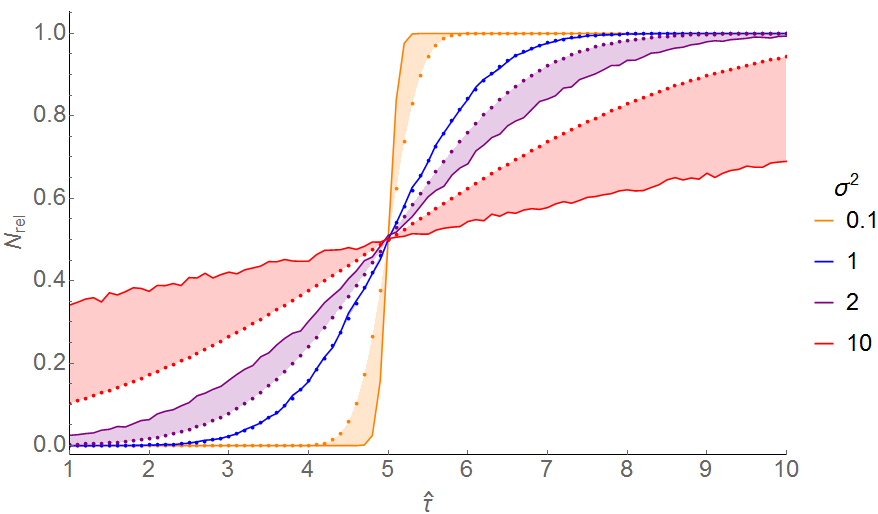
\includegraphics[width=.65\columnwidth]{../assets/thm2fig.png}
	\centering\caption{Visualization of Theorem~\ref{thrm:relativefrequency} as $N_{rel}$ estimates $\Phi(\cdot)$. The plot was generated by running Eqn.~\ref{eqn:Nrel} 10,000 times for each point in $\hat{\tau} = [1,10,\text{ (inc.) }0.1]$. $n = 10$, $\td = 5$ and $x_i = \hat{\tau} + \eta_i$ ($\eta_i \sim\mathcal{N}(0, \sigma)$). Each curve in the plot is generated by sweeping $\sigma = \{0, 0.1, 1, 2, 10\}$, with $\sigma = 0$ being a step-function and $\sigma = 10$ having the \emph{flattest} slope.}\vspace{-10px}\label{fig:thm2fig}
\end{figure}

Therefore, for large $n$, the relative frequency of agents taking part in the activity has a shape that follows the shape of the cdf of a standard Gaussian random variable, as seen in Fig.~\ref{fig:thm2fig}, i.e. agents may use deterministic threshold strategies but their aggregate behavior would appear to follow such a continues (sigmoid) threshold.

The final step to explain the prevalence of sigmoid functions in multiagent settings is to note that:
\begin{align*}
|\Phi(\frac{\hat{\tau}-\td}{\sigma^2})-\frac{1}{1+e^{-d(\frac{\hat{\tau}-\td}{\sigma^2})}}|\leq 0.01,
\end{align*}
for all $\hat{\tau}\in\R$ and some optimal value $d\approx 1.704$ (see \cite{camilli1994} and the references therein for the details of this approximation). This means that the aggregate behavior of the agents following deterministic threshold policies would (almost) follow the shape of a logistic sigmoid function whose drift is directly proportional to $\td$ and the slope  is inversely proportional to $\sigma^2$. 

\section{Discussion and Summary}\label{sec:discsum}
I show in Theorem~\ref{thrm:mainthrm} that a communication-free agent-level threshold strategy is sufficient and necessary to achieve a TA resulting in system-level equilibrium for concurrent benefit tasks. I then show in Theorem~\ref{thrm:relativefrequency} how such a policy effectively reduces to a continuous threshold response function that is commonly observed in social insects. While this result explains why one would observe such phenomena in natural systems, the game theory perspective leaves it unclear why one should choose a continuous threshold function in a robotic setting. Here, recall that a benefit of using CRT vs.~DRT is the randomness it adds, allowing swarm systems to quickly adapt to changes in task and environment parameters \cite{Bonabeau1997}. In particular, deliberately tuning the slope of the sigmoid threshold function as I have investigated in \cite{Kanakia2014} allows a swarm to explore different team sizes, and possibly learn from this experience, an aspect I wish to study in future work (see Chapter~\ref{ch:optimization}). 

Theorem~\ref{thrm:mainthrm} states that there exists a unique strategy profile $s$ such that it is a system-level Bayesian Nash Equilibrium for all agents performing a concurrent benefit task. Notice that this theorem makes no claims towards an \emph{optimal} strategy for TA, just an equilibrium strategy. It is important to distinguish between these two properties of the swarm system. Clearly, optimal outcomes will require communication among agents or, at least, a central entity with access to global information. In in the next chapter I the area in-between where agents exchange limited amounts of information, such as their noisy estimates $x_i$.

This raises the question what ``communication'' and ``sharing of information'' actually mean. In this chapter, communication is limited to common observations of an unknown environmental variable $\tau$. Natural swarming systems often communicate by modifying the environment, a form of indirect communication known as stigmergy \cite{Grasse1959}. The key difference between this form of communication and direct exchange of information, as I discuss in \cite{Touri2014}, is that the same information is simultaneously accessible to all individuals. I therefore believe that the results presented here extend also to indirect communication via stigmergy where $\tau$ is the measurable result of previous agent activity.



%%%%%%%%%%%%%%%%%%%%%%%%%%%%%%%%%%%%%%%%%%%%%%%%%%%%%%%%%%%%%%%%%%%%%%%%%%%%%%%%
\chapter{Designing an Optimal Control Model for Multi-Agent Systems}\label{ch:optimization}
Finally, building off my results from the previous two chapters, this chapter describes a particular methodology for designing, controlling and optimizing swarm robot controllers. While this is by no means the only modeling method available for robot swarms---e.g., other (related) modeling and control methods are described in \cite{Bayazit2005,Berman2007,Billard1999,Sugawara2013}---it has the important property of being an iterative method that integrates multiple levels of abstraction of the multi-agent system. This opens up the opportunity for simultaneous parameter discovery and optimization, as seen in the next section.

\section{Iterative Least-Squares Optimization}\label{sec:opt}
I can re-write the rate equations in~\eqref{eq:rateeqns} (see Chapter~\ref{ch:background} for more information) as,
\begin{equation}
S'(\theta,\mu,t) = \Gamma\left(\vec{S}, \theta, \mu, t\right)
\end{equation}
So the temporal evolution of a model is characterized by its state in the past, $\vec{S}(t)$, partially known system parameters ($\theta$), robot control parameters ($\mu$), and time. In other words, the probabilities in eq.\eqref{eq:rateeqns} and eq.\eqref{eq:master} need not be constant values but functions of $\theta$, $\mu$, and $t$.

Two situations commonly arise when designing macro-level models for swarm systems. Firstly, there is the problem of identifying the important system parameters, $\theta$. As pointed out in\cite{Correll2008}, ``In a real robotic system, not all of the model parameters can be known beforehand, either due to uncertainty of measurements or because the chosen model oversimplifies the system (e.g., ignoring friction or sensor noise).'' As such, these parameters are estimated from observations of real experiments and require solving the following optimization problem.
\begin{equation}
	\theta^* = \underset{\overline{\theta}}{\argmin}\left(S^*(\overline{\theta},\mu) - \hat{S}^*(\theta, \mu)\right)^2 \label{eq:thetaopt}
\end{equation}
$S^*(\overline{\theta},\mu)$ is the model prediction of the state vector at steady-state,\\ i.e.~$S^*(\overline{\theta},\mu) = \lim_{t \to \infty}S(\overline{\theta},\mu, t)$, and $\hat{S}^*(\theta, \mu)$ is the experimentally observed state vector at steady-state.

The second situation involves finding optimal control parameters, $\mu$, for a known set of system parameters, $\theta$. The goal is to drive the system towards a desired steady-state distribution, $\tilde{S}^*$, by tuning the model's control parameters. The is accomplished by solving the following optimization problem.
\begin{equation}
	\mu^* = \underset{\overline{\mu}}{\argmin}\left(\tilde{S}^* - S^*(\theta, \overline{\mu})\right)^2 \label{eq:muopt}
\end{equation}

It is evident from eq.\eqref{eq:thetaopt} and eq.\eqref{eq:muopt} that these separate optimization problems are not independent. Starting with initial guesses $\mu(0)$ and $\theta(0)$ alongside simulation results from these guesses, one can generate increasingly better values of $\theta$ and $\mu$ for the desired final state distribution $\tilde{S}^*$ using the following recurrence relations.
\begin{align}\label{eq:paramrel}
	\overline{\theta}(n + 1) = & \underset{\overline{\theta}}{\argmin}\sum\limits_{i=0}^{n}\left(S^*(\overline{\theta},\overline{\mu}(i)) - \hat{S}^*(\theta, \overline{\mu}(i), i)\right)^2\\
	\overline{\mu}(n + 1) = & \underset{\overline{\mu}}{\argmin}\left(\tilde{S}^* - S^*(\overline{\theta}(n + 1), \mu)\right)^2
\end{align}
The index $n$ corresponds to the number of the experiment that led to an observation of the steady state $\hat{S}^*(\theta, \mu, n)$. Further discussion and applications of this parameter optimization approach are discussed in\cite{Correll2006a,Correll2008}.

\begin{figure}[!ht]
\centering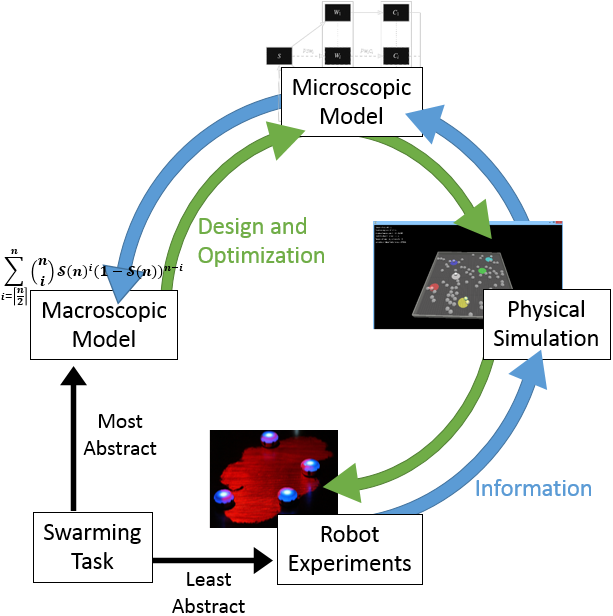
\includegraphics[width=.75\textwidth]{../assets/ssmodel.png}
\centering\caption{The closed loop design framework for a swarm robot system controller. Real world data is passed through models running at different layers of abstraction, which in-turn feed their solutions for parameter discovery and optimization back to the real system.}\label{fig:recipe}
\end{figure}

I have now discussed all the of the steps needed to design a robot controller and its corresponding (non-spatial) models for a particular swarming task. Figure~\ref{fig:recipe} gives us a visual representation of the entire process including the modeling methods used at different levels of abstraction of the swarm system. This design methodology is a closed loop feedback system. Setting up the required swarming task as a real physical experiment or physical simulation allows us to discover and measure the different free parameters in the system. I then use these variables in lower resolution models (micro-level) as well as in the development of mathematical models (macro-level) for my system. These more abstract models allow us to rapidly experiment with system parameters and optimize them. I can then use these optimized parameters back in the real physical experiments to improve the desired behavior of the system and repeat the cycle till the desired level of accuracy and satisfaction of  model behavior is achieved.

\begin{figure}[!tb]
\centering\begin{subfigure}{.6\textwidth}
	\centering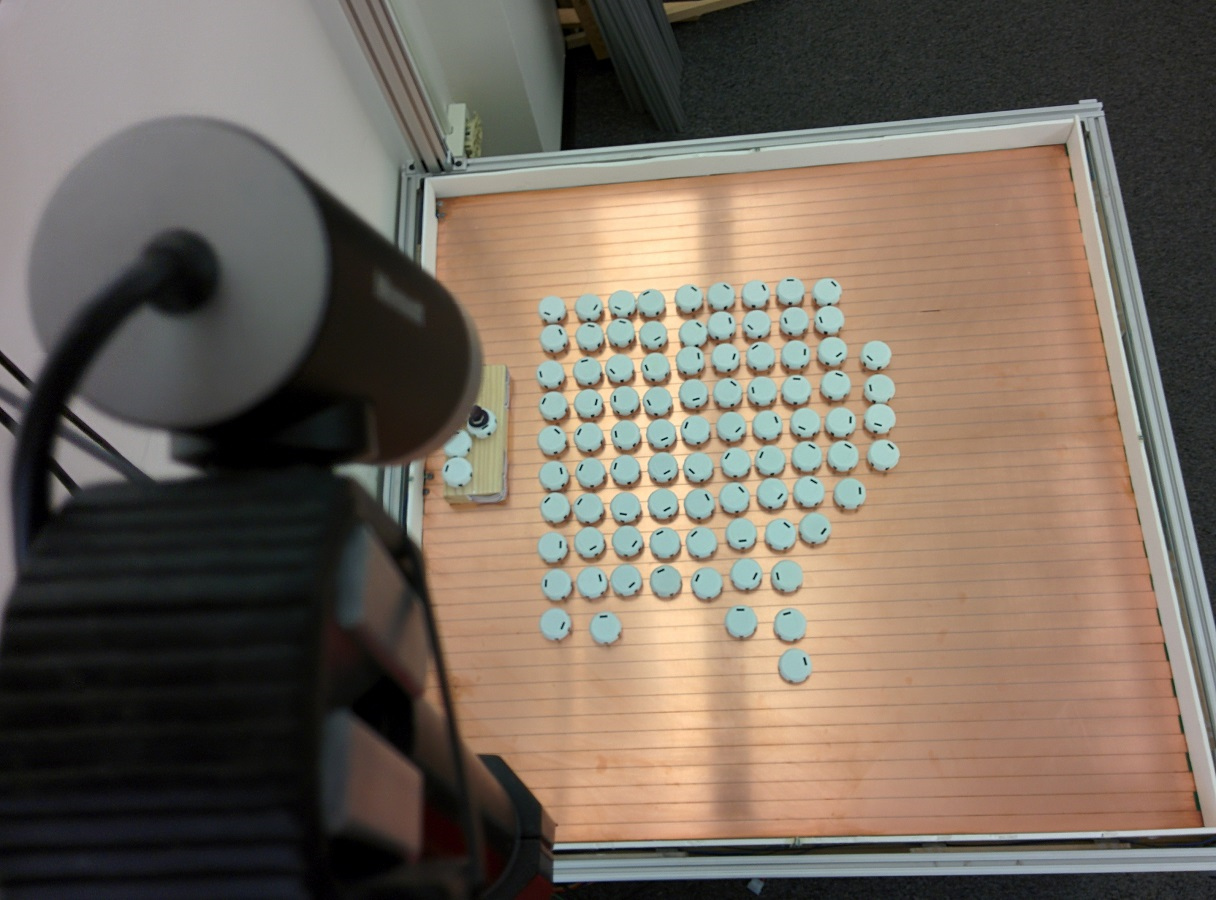
\includegraphics[scale=.275]{../assets/droplettablewc.png}
\end{subfigure}~
\centering\begin{subfigure}{.4\textwidth}
	\centering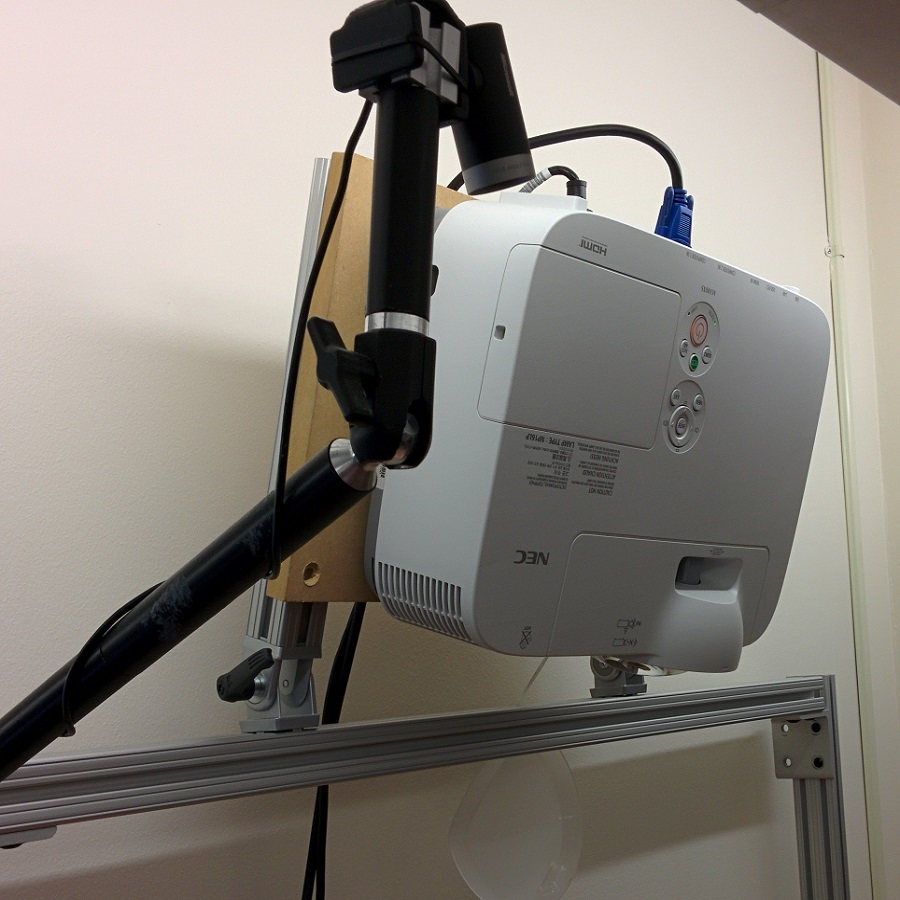
\includegraphics[scale=.275]{../assets/droplettablepj.png}
\end{subfigure}
\centering\caption{(Left) The droplet platform from the point-of-view of an overhead webcam. (Right) The overhead projector setup for Droplet testing and experimentation.}
\end{figure}\label{fig:optexpsetup}

I propose the following experiment for validating all the research I have done so far. Going back to my firefighting example (See Figures~\ref{fig:dropletfire} and \ref{fig:ggsetup}) and the work discussed in Chapter~\ref{ch:resthmodel}, the free parameters of the swarm system are $\theta$ and $\tau$ that map to the desired mean team size and variance at a fire. In the experiment, each robot would make it's own initial guess for these two parameters and then a series of PFSM models and rate equation solutions (running on a PC, offline from the robot hardware) would iteratively compute the expected ``best'' team size for a fire of a certain size. This updated parameter information is communicated to the swarm through the use of infrared communication channels and the robots update their estimates of the control parameters while sending back sensory information (environment parameters) through the same channels to a central controller. The magnitude of the fire is controlled by projecting blobs of different color gradients (from red being hottest to yellow being coldest) onto the Droplet arena from a computer program attached to the projector. An objective function must be chosen for optimizing the system and this is a problem I am currently working on. My work in Chapter~\ref{ch:existeqrtm} will be very helpful on this front as the expectation of equilibrium in a swarm system using a CRT model for TA could lead to a well defined notion of system-level optimality. The reader should bear in mind that equilibrium and optimality are not often related in the sort of complex systems we are interested in here but there are notions of how good an equilibrium strategy is compared to an optimal strategy in game theory that could prove useful to my cause. Refer to \cite{Koutsoupias1999} and Section~\ref{sec:poapos} for more information on this topic. Formally defining the optimum behavior for a swarm system is an still an open problem that needs further study. 

A MAS can be made to behave in a desired manner using the approach mentioned above but it is a centralized approach. There exist distributed optimization strategies such as the sub-gradient methods discussed in \cite{Nedic2009}. These methods may lead to a distributed strategy for optimal control of a MAS and, time permitting, bear further investigation. An avenue for analyzing the benefits vs.~payoffs for centralized vs.~decentralized systems is once again afforded to us by game theory. The following \emph{addendum section} describes some work I have done in this regard.

\chapter{\textbf{Addendum}: Optimal Vehicle-Target Assignment}
This section provides a brief overview of some---as yet unsubstantiated---work I did formulating the TA problem for MAS as a vehicle-target assignment problem that is well known in game theory. The advantages this approach provides are strict bounds on how well a centralized vs.~decentralized system can perform, given a set of constraints. Formulating TA as target assignment provides a direct analogy to the \emph{0-1 Integer Knapsack Problem} which indicates that no polynomial time algorithm is currently known to solve the proposed problem, albeit, the additional constraints imposed by a real robotic system may in-fact provide a fast solution.

I inspect the cooperative, distributed welfare game of vehicle-target assignment with welfare functions that are not sub-modular, but are instead based on target specific threshold values and player-target assignment constraints. Target threshold values define individual agent payoffs depending on the size of the group. One can imagine cooperative scenarios where a group must attain at least some minimum size to successfully complete a task. Tasks such as real-time mapping, object detection and containment, etc. fall into this category. Such tasks can often be seen as a special flavor of the vehicle-target assignment problem where players groups of a certain size  must pick the same target to successfully complete their mission and receive a non-zero payoff.

Most recent work in distributed welfare games\cite{Marden2008, Marden2013} assumes that players are, in general, non-cooperative. While a comprehensive study of the vehicle-target assignment problem has been done by Arslan et al.\cite{Arslan2007}, the authors do not discuss the specific scenario discussed in this section. Since target thresholds remove the submodularity property from welfare functions for this game, work on valid utility games by Vetta et al.\cite{Vetta2002} cannot be used in this circumstance and additional analysis must be done to predict bounds on PoA/PoS.

\section{Problem Setup and Example}
The cooperative game is set up as follows:
\begin{itemize}
	\item Players: $\Pl = \{1,2,3,\ldots, N\}$.
	\item Targets: $t \in \Ta$, $|\Ta| = M$.
	\item Target Threshold: $k_t$, $t \in \Ta$.
	\item Player Constraints: $c_i = S \subseteq \Ta$, $c_i \in C$.
	\item Target Detection Probability: We assume all players can perfectly detect and assign themselves to targets within their constraints, $c_i$. Therefore detection probability for all targets is 1.
	\item Target specific welfare function, 
\begin{align}
	W_t(|a|_t) & = \left\{
	\begin{array}{ll}
		1 & |a|_t \geq k_t\\
		0 & o/w
	\end{array}\right.\label{eq:wf}
\end{align}
	\item Global welfare function,
\begin{align}
	W(a) = \sum\limits_{t \in \Ta} W_t(|a|_t)\label{eq:gwf}
\end{align}
\end{itemize}
We can clearly see that the welfare function, $W(|a|_t)$, is not submodular. The fact that the global welfare function is just an accumulator of ``successfully assigned'' targets does help with PoA/PoS analysis.

\textbf{Definition:} A target is considered ``successfully assigned'' when $|a|_t \geq k_t$, i.e. the number of player's assigned to it is greater than or equal to its threshold value.

\textbf{Definition:} A target is considered ``perfectly assigned'' when $|a|_t = k_t$.

The following example describes a cooperative game with target thresholds and player constraints as seen in Figure \ref{fig:ex1}.
\begin{itemize}
	\item Players: $\Pl = \{1,2,3,4\}$
	\item Targets: $t \in \Ta = \{a, b, c\}$
	\item Target Threshold: $k_a = k_b = k_c = 2$
	\item Target specific welfare function, $W_t(|a|_t)$, from \eqref{eq:wf}
	\item Anonymous Global welfare function, $W(a) = \sum\limits_{t \in \Ta} W_t(|a|_t)$, from \eqref{eq:gwf}.
\end{itemize}
\begin{figure}[!htb]
	\centering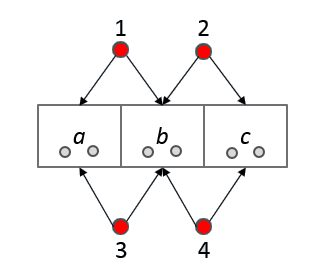
\includegraphics[width=5.5cm]{../assets/ex1.png}
	\centering\caption{A cooperative game with 4 players and 3 targets. Gray pegs indicate the target's minimum threshold value while the arrows depict player assignment constraints.}\label{fig:ex1}
\end{figure}

Global welfare values for this example are listed in Table \ref{tab:mcgw}. Note that these values depend only on the number of successfully assigned targets. 
\begin{table}[!htb]
	\centering\begin{tabular}{r|c|c|}
	\multicolumn{1}{c}{}
	& \multicolumn{1}{c}{b}
	& \multicolumn{1}{c}{$c$}\\
	\cline{2-3}
	$a$ & $2$ & $1$\\
	\cline{2-3}
	$b$ & $1$ & $1$\\
	\cline{2-3}
	\multicolumn{1}{c}{}
	& \multicolumn{2}{c}{$a,b$}
	\end{tabular}~
	\centering\begin{tabular}{r|c|c|}
	\multicolumn{1}{c}{}
	& \multicolumn{1}{c}{$b$}
	& \multicolumn{1}{c}{$c$}\\
	\cline{2-3}
	$a$ & $1$ & $2$\\
	\cline{2-3}
	$b$ & $1$ & $1$\\
	\cline{2-3}
	\multicolumn{1}{c}{}
	& \multicolumn{2}{c}{$a,c$}
	\end{tabular}~
	\centering\begin{tabular}{r|c|c|}
	\multicolumn{1}{c}{}
	& \multicolumn{1}{c}{$b$}
	& \multicolumn{1}{c}{$c$}\\
	\cline{2-3}
	$a$ & $1$ & $1$\\
	\cline{2-3}
	$b$ & $1$ & $1$\\
	\cline{2-3}
	\multicolumn{1}{c}{}
	& \multicolumn{2}{c}{$b,b$}
	\end{tabular}~
	\centering\begin{tabular}{r|c|c|}
	\multicolumn{1}{c}{}
	& \multicolumn{1}{c}{$b$}
	& \multicolumn{1}{c}{$c$}\\
	\cline{2-3}
	$a$ & $1$ & $1$\\
	\cline{2-3}
	$b$ & $1$ & $2$\\
	\cline{2-3}
	\multicolumn{1}{c}{}
	& \multicolumn{2}{c}{$b,c$}
	\end{tabular}
	\centering\caption{Global welfare for the vehicle-target assignemt example scenario with target thresholds and player constraints.}\label{tab:mcgw}
\end{table}

\section{Selecting Utility Functions}
We discuss the effects that choosing different utility functions has for this example scenario. We discuss two utility functions, marginal contribution and Shapley value utility, and apply log-linear learning to observe equilibria of the system under both utility design choices.

\subsection{Marginal Contribution (MC) Utility}
MC utility gives us two important and desirable properties for a good utility function, existence and efficiency of NE. NE existence is guaranteed because the chosen binary welfare function is anonymous and  depends only on the number of vehicles assigned to a target\cite{Monderer1996}. Given that the global objective function is just a counting function that counts the total number of successfully assigned targets, we can show that a maximum assignment is always an NE of the system as it results in maximum player payoffs (see proof in \textbf{Price of Stability} section). Player utility values using MC utility are listed in Table \ref{tab:mcUtil}.  

\begin{table}[!htb]
	\centering\begin{tabular}{r|c|c|}
	\multicolumn{1}{c}{}
	& \multicolumn{1}{c}{b}
	& \multicolumn{1}{c}{$c$}\\
	\cline{2-3}
	$a$ & \textcolor{blue}{$1,1,1,1$} & $1,1,0,0$\\
	\cline{2-3}
	$b$ & $0,0,0,0$ & \textcolor{red}{$1,0,0,1$}\\
	\cline{2-3}
	\multicolumn{1}{c}{}
	& \multicolumn{2}{c}{$a,b$}
	\end{tabular}~
	\centering\begin{tabular}{r|c|c|}
	\multicolumn{1}{c}{}
	& \multicolumn{1}{c}{$b$}
	& \multicolumn{1}{c}{$c$}\\
	\cline{2-3}
	& $1,0,1,0$ & \textcolor{blue}{$1,1,1,1$}\\
	\cline{2-3}
	& \textcolor{red}{$1,1,0,0$} & $0,1,0,1$\\
	\cline{2-3}
	\multicolumn{1}{c}{}
	& \multicolumn{2}{c}{$a,c$}
	\end{tabular}~
	\centering\begin{tabular}{r|c|c|}
	\multicolumn{1}{c}{}
	& \multicolumn{1}{c}{$b$}
	& \multicolumn{1}{c}{$c$}\\
	\cline{2-3}
	& $0,0,0,0$ & \textcolor{red}{$0,0,1,1$}\\
	\cline{2-3}
	& \textcolor{red}{$0,0,0,0$} & $0,0,0,0$\\
	\cline{2-3}
	\multicolumn{1}{c}{}
	& \multicolumn{2}{c}{$b,b$}
	\end{tabular}~
	\centering\begin{tabular}{r|c|c|}
	\multicolumn{1}{c}{}
	& \multicolumn{1}{c}{$b$}
	& \multicolumn{1}{c}{$c$}\\
	\cline{2-3}
	& \textcolor{red}{$0,1,1,0$} & $0,1,0,1$\\
	\cline{2-3}
	& $0,0,0,0$ & \textcolor{blue}{$1,1,1,1$}\\
	\cline{2-3}
	\multicolumn{1}{c}{}
	& \multicolumn{2}{c}{$b,c$}
	\end{tabular}
	\centering\caption{Player payoffs for the example scenario using Marginal Contribution utility.}\label{tab:mcUtil}
\end{table}

Averaging over 1000 runs of log-linear learning for 1000 iterations each and using temperature $T = 0.15$, the following stationary distribution is observed (Table \ref{tab:mcsd}).

\begin{table}[!htb]
	\centering\begin{tabular}{r|c|c|}
	\multicolumn{1}{c}{}
	& \multicolumn{1}{c}{b}
	& \multicolumn{1}{c}{$c$}\\
	\cline{2-3}
	$a$ & \textcolor{blue}{$0.343$} & $0.000$\\
	\cline{2-3}
	$b$ & $0.002$ & \textcolor{red}{$0.000$}\\
	\cline{2-3}
	\multicolumn{1}{c}{}
	& \multicolumn{2}{c}{$a,b$}
	\end{tabular}~
	\centering\begin{tabular}{r|c|c|}
	\multicolumn{1}{c}{}
	& \multicolumn{1}{c}{$b$}
	& \multicolumn{1}{c}{$c$}\\
	\cline{2-3}
	& $0.001$ & \textcolor{blue}{$0.308$}\\
	\cline{2-3}
	& \textcolor{red}{$0.000$} & $0.000$\\
	\cline{2-3}
	\multicolumn{1}{c}{}
	& \multicolumn{2}{c}{$a,c$}
	\end{tabular}~
	\centering\begin{tabular}{r|c|c|}
	\multicolumn{1}{c}{}
	& \multicolumn{1}{c}{$b$}
	& \multicolumn{1}{c}{$c$}\\
	\cline{2-3}
	& $0.000$ & \textcolor{red}{$0.001$}\\
	\cline{2-3}
	& \textcolor{red}{$0.000$} & $0.000$\\
	\cline{2-3}
	\multicolumn{1}{c}{}
	& \multicolumn{2}{c}{$b,b$}
	\end{tabular}~
	\centering\begin{tabular}{r|c|c|}
	\multicolumn{1}{c}{}
	& \multicolumn{1}{c}{$b$}
	& \multicolumn{1}{c}{$c$}\\
	\cline{2-3}
	& \textcolor{red}{$0.000$} & $0.000$\\
	\cline{2-3}
	& $0.000$ & \textcolor{blue}{$0.345$}\\
	\cline{2-3}
	\multicolumn{1}{c}{}
	& \multicolumn{2}{c}{$b,c$}
	\end{tabular}
	\centering\caption{Stationary Distribution approximated using log-linear learning and MC utility.}\label{tab:mcsd}
\end{table}

As is evident from these results, applying log-linear learning using MC utility converges the system to perfect target assignment if a perfect assignment can be made. The NE in blue are all cases of perfect assignment while the equilibria in red are cases of successful assignment but do not maximize global welfare. We now look at what happens when Shapley value utility is used instead of MC for this game.

\subsection{Shapley Value (SV) Utility}
Using SV utility, each player's utility for selecting target, $t \in \Ta$, can be computed using the simplified equation,
\begin{align}
	U_i(t, a_{-i}) & = \left\{
		\begin{array}{ll}	
			1/|a|_t & |a|_t \geq k_t\\
			0 & |a|_t < k_t
		\end{array}\right.
\end{align}

Player utility values are listed in Table \ref{tab:svUtil}. Once again, running log-linear learning with the same parameters as used for marginal contribution utility we see the following stationary distribution (Table \ref{tab:svsd}).
\begin{table}[!htb]
	\centering\begin{tabular}{r|c|c|}
	\multicolumn{1}{c}{}
	& \multicolumn{1}{c}{b}
	& \multicolumn{1}{c}{$c$}\\
	\cline{2-3}
	$a$ & \textcolor{blue}{$\frac{1}{2},\frac{1}{2},\frac{1}{2},\frac{1}{2}$} & $\frac{1}{2},0\frac{1}{2},0$\\
	\cline{2-3}
	$b$ & $\frac{1}{3},\frac{1}{3},0,\frac{1}{3}$ & \textcolor{red}{$\frac{1}{2},0,0,\frac{1}{2}$}\\
	\cline{2-3}
	\multicolumn{1}{c}{}
	& \multicolumn{2}{c}{$a,b$}
	\end{tabular}~
	\centering\begin{tabular}{r|c|c|}
	\multicolumn{1}{c}{}
	& \multicolumn{1}{c}{$b$}
	& \multicolumn{1}{c}{$c$}\\
	\cline{2-3}
	& $\frac{1}{2},0,\frac{1}{2},0$ & \textcolor{blue}{$\frac{1}{2},\frac{1}{2},\frac{1}{2},\frac{1}{2}$} \\
	\cline{2-3}
	& \textcolor{red}{$\frac{1}{2},\frac{1}{2},0,0$} & $0,\frac{1}{2},0\frac{1}{2}$ \\
	\cline{2-3}
	\multicolumn{1}{c}{}
	& \multicolumn{2}{c}{$a,c$}
	\end{tabular}~
	\centering\begin{tabular}{r|c|c|}
	\multicolumn{1}{c}{}
	& \multicolumn{1}{c}{$b$}
	& \multicolumn{1}{c}{$c$}\\
	\cline{2-3}
	& $0,\frac{1}{3},\frac{1}{3},\frac{1}{3}$ & \textcolor{red}{$0,0,\frac{1}{2},\frac{1}{2}$}\\
	\cline{2-3}
	& \textcolor{red}{$\frac{1}{4},\frac{1}{4},\frac{1}{4},\frac{1}{4}$} & $\frac{1}{3},0,\frac{1}{3},\frac{1}{3}$\\
	\cline{2-3}
	\multicolumn{1}{c}{}
	& \multicolumn{2}{c}{$b,b$}
	\end{tabular}~
	\centering\begin{tabular}{r|c|c|}
	\multicolumn{1}{c}{}
	& \multicolumn{1}{c}{$b$}
	& \multicolumn{1}{c}{$c$}\\
	\cline{2-3}
	& \textcolor{red}{$0,\frac{1}{2},\frac{1}{2},0$} & $0,\frac{1}{2},0,\frac{1}{2}$\\
	\cline{2-3}
	& $\frac{1}{3},\frac{1}{3},\frac{1}{3},0$ & \textcolor{blue}{$\frac{1}{2},\frac{1}{2},\frac{1}{2},\frac{1}{2}$}\\
	\cline{2-3}
	\multicolumn{1}{c}{}
	& \multicolumn{2}{c}{$b,c$}
	\end{tabular}
	\centering\caption{Player payoffs using Shapley Value utility.}\label{tab:svUtil}
\end{table}
\begin{table}[!htb]
	\centering\begin{tabular}{r|c|c|}
	\multicolumn{1}{c}{}
	& \multicolumn{1}{c}{b}
	& \multicolumn{1}{c}{$c$}\\
	\cline{2-3}
	$a$ & \textcolor{blue}{$0.175$} & $0.004$\\
	\cline{2-3}
	$b$ & $0.055$ & \textcolor{red}{$0.005$}\\
	\cline{2-3}
	\multicolumn{1}{c}{}
	& \multicolumn{2}{c}{$a,b$}
	\end{tabular}~
	\centering\begin{tabular}{r|c|c|}
	\multicolumn{1}{c}{}
	& \multicolumn{1}{c}{$b$}
	& \multicolumn{1}{c}{$c$}\\
	\cline{2-3}
	& $0.003$ & \textcolor{blue}{$0.159$}\\
	\cline{2-3}
	& \textcolor{red}{$0.004$} & $0.005$\\
	\cline{2-3}
	\multicolumn{1}{c}{}
	& \multicolumn{2}{c}{$a,c$}
	\end{tabular}~
	\centering\begin{tabular}{r|c|c|}
	\multicolumn{1}{c}{}
	& \multicolumn{1}{c}{$b$}
	& \multicolumn{1}{c}{$c$}\\
	\cline{2-3}
	& $0.057$ & \textcolor{red}{$0.002$}\\
	\cline{2-3}
	& \textcolor{red}{$0.266$} & $0.046$\\
	\cline{2-3}
	\multicolumn{1}{c}{}
	& \multicolumn{2}{c}{$b,b$}
	\end{tabular}~
	\centering\begin{tabular}{r|c|c|}
	\multicolumn{1}{c}{}
	& \multicolumn{1}{c}{$b$}
	& \multicolumn{1}{c}{$c$}\\
	\cline{2-3}
	& \textcolor{red}{$0.005$} & $0.004$\\
	\cline{2-3}
	& $0.056$ & \textcolor{blue}{$0.154$}\\
	\cline{2-3}
	\multicolumn{1}{c}{}
	& \multicolumn{2}{c}{$b,c$}
	\end{tabular}
	\centering\caption{Stationary Distribution approximated using log-linear learning and SV utility.}\label{tab:svsd}
\end{table}

In this case, the worst NE has the highest likelihood of being chosen by log-linear learning. The case when all the agents are assigned to the same target ($b, b, b, b$) results in both, minimum player utility as well as the lowest global welfare but is still an equilibrium of the game. While one can argue that the ``good'' equilibria---with equal global welfare and player payoffs---are collectively more likely to occur compared to the one bad equilibrium, this is still a $\approx 2:1 ((.175 + .159 + .154) / .266)$ ratio.

In this example case it is clearly a better idea to use MC over SV when picking an appropriate utility function for this system to do optimal target assignment.

\section{Price of Anarchy/Stability Analysis}\label{sec:poapos}
PoA for this game is only defined under specific conditions for this vehicle-target assignment problem. The global welfare for the worst NE of the game can be $W_{NE}^{bad} = 0$, e.g. $|\Pl| = 3$, $|\Ta| = 3$, $c_i = \Ta$ $\forall i \in \Pl$, $k_t = 3$ $\forall t \in \Ta$. If every agent is assigned a unique target in this situation, then the system is at an equilibrium and no agent has any incentive to unilaterally deviate since they cannot improve their respective payoff or the global system welfare. In such a situation $W_{NE} = 0$ and thus $PoA = W_{OPT} / W_{NE}^{bad}$ would be undefined (or infinite).

In general, $W_{NE}^{bad} \not= 0$ when: for all actions in the valid action set, there must exist a target-$t$ such that it is either successfully assigned or is one agent away from being successfully assigned and an agent-$p$ exists that is not assigned to $t$ in the current action but has $t$ in it's target constraint set ($t \in c_p$, $a_p \not= t$).
\begin{align}
	\forall a \in 2^\Co, \exists t \in \Ta \text{ s.t. } |a|_t \geq (k_t - 1)\label{eq:poa}
\end{align}

If the property \eqref{eq:poa} holds for a given game then its PoA is bounded; $1 \leq PoA \leq W_{OPT}$. As more agents are ``added'' to the game (effectively creating a new game), the PoA goes down from $W_{OPT}$ to 1 when $|\Pl| \geq \sum\limits_{t \in \Ta} k_t$ (see Figure \ref{fig:poa}).

\begin{figure}[!htb]
	\centering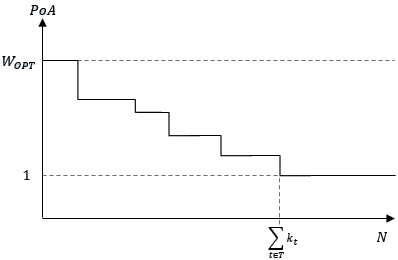
\includegraphics[width=7.5cm]{../assets/poa.png}
	\centering\caption{Bounds on PoA as $|\Pl|$ increases.}\label{fig:poa}
\end{figure}

PoS for this game is always 1. To prove this, assume we start with an action $a^{OPT}$ which results in optimal global welfare $W_{OPT}$. I will prove that this action $a^{OPT}$ must also be NE$^{best}$. If a player decides to unilaterally deviate from $a^{OPT}$ to $a'$ then $U_i(a'_i, a'_{-i}) > U_i(a^{OPT}_i, a^{OPT}_{-i})$. This means that the target $a'_i$ must not have been optimally assigned for action $a^{OPT}$. It is easy to see that a player's utility can only be increased if they move between successfully assigned targets or from some target (not necessarily successfully assigned) to a successfully assigned target. This results in one of two scenarios, either target $a^{OPT}_i$ was successfully assigned before the switch and is no longer successfully assigned in action $a'$ or both targets $a^{OPT}_i$ and $a'_i$ are successfully assigned in $a'$. 

If the first case is true then that means target $a'_i$ was successfully assigned in action $a'$ by the switch from player-$i$ but was not successfully assigned in action $a^{OPT}$ (this is the only way player-$i$ could receive a better payoff for deviating from $a^{OPT}$). This means the global welfare is reduced by 1 and increased by one when going from $a^{OPT}$ to $a'$ which means $a'$ is another optimal action and we can replace our starting action with this new one and continue this recursive argument.

If the second case is true then player-$i$ switch did nothing to the global welfare and we can once again replace $a^{OPT}$ with $a'$ and continue this argument.

Finally, if this player's deviation from $a^{OPT}$ to $a'$ resulted in a better payoff for any other reason, it means the new target chosen $a'_i$ was not successfully assigned in action $a^{OPT}$ but has been successfully assigned in action $a'$. This would imply $W(a') > W(a^{OPT})$ since action $a'$ now has one new successfully assigned target, $a'_i$. This would result in a contradiction since that would imply $a^{OPT}$ was never an optimum. Which means that no player-$i$ would deviate from $a^{OPT}$ for any reason, thereby making $a^{OPT}$ a NE. $a^{OPT}$ is also the best NE, $W(a^{OPT}) = W_{NE}^{best}$ by it's very definition and so PoS for this game is always 1.

\section{Finding Optimal Welfare}
Since the global welfare function is essentially a counting function (1 for targets that have been successfully assigned, 0 otherwise), it is maximized by maximizing the number of successfully assigned targets.

In the simplistic case when $k_t = k$ $\forall t \in \Ta$, and $c_i = \Ta$ $\forall i \in \Pl$, the maximum welfare is,
\begin{align}
	W^{OPT} & = \left\{
	\begin{array}{ll}
		\floor*{\frac{N}{k}} & M \geq N/k\\
		M & o/w
	\end{array}
	\right.\notag\\
	& = \min\left(\left\lfloor\frac{N}{k}\right\rfloor, M\right)
\end{align}

In the more complex case when $k_t$'s are not all the same value, the optimal welfare is found by maximizing the number of targets that can be successfully assigned. This is equivalent to a well studied problem in computer science called the \textbf{0-1 Integer Knapsack Problem} which, when posed as an optimization problem, is known to be NP-hard. I have not formally worked out the reduction from target assignment to knapsack but would be excited to do so, given enough time. This means that no polynomial time (in M) algorithm exists that can assign players to targets to maximize system utility---which makes finding $W^{OPT}$ and in turn, PoA/PoS for this game, a difficult problem for large values of $M$. For many practical purposes, a pseudo-polynomial time algorithm exists to solve the knapsack problem.

Finally, re-introducing player constraints makes finding $W_{OPT}$ an even more complicated affair and I have not studied this further, as yet. This would be a good future direction to take this preliminary work in.

There are a number of further questions one can ask about the class of games discussed in this section. My goal was mainly to show that game theory can be a viable alternative means to study cooperative scenarios with the system restrictions mentioned in this paper. While my bounds on PoA are not particularly satisfying, and rather obviously inferred just by thinking about such systems, perhaps a deeper analysis of the problem can provide exact values for PoA under special conditions\ldots Probably involving ratios between $|\Pl|$, $|\Ta|$ and $k_t$.



%%%%%%%%%%%%%%%%%%%%%%%%%%%%%%%%%%%%%%%%%%%%%%%%%%%%%%%%%%%%%%%%%%%%%%%%%%%%%%%%
%%%%%%%%%   The Bibliography, if any   %%%%%%%%%
\bibliographystyle{ieeetr}		% or "plain", "siam", or "alpha", etc.
%\nocite{*}						% list all refs in database, cited or not
\bibliography{../refworks}
\end{document}

\end{document}


